\documentclass[10pt,letterpaper]{article}
\usepackage[top=0.85in,left=2.00in,footskip=0.75in]{geometry}

% Use adjustwidth environment to exceed column width (see example table in text)
\usepackage{changepage}

% Use Unicode characters when possible
\usepackage[utf8]{inputenc}

% textcomp package and marvosym package for additional characters
\usepackage{textcomp,marvosym}

% fixltx2e package for \textsubscript
\usepackage{fixltx2e}
%\usepackage{subcaption}

%\usepackage{subfig}
% amsmath and amssymb packages, useful for mathematical formulas and symbols
\usepackage{amsmath,amssymb}

% cite package, to clean up citations in the main text. Do not remove.
\usepackage{cite}

%lstlisting
\usepackage{listings}

% Use nameref to cite supporting information files (see Supporting Information section for more info)
\usepackage{nameref}
%\usepackage{hyperref}

% line numbers
\usepackage[right]{lineno}

% ligatures disabled
\usepackage{microtype}
%\DisableLigatures[f]{encoding = *, family = * }

% rotating package for sideways tables
\usepackage{rotating}

% Remove comment for double spacing
%\usepackage{setspace} 
%\doublespacing

%subfigures
\usepackage[lofdepth,lotdepth]{subfig}
% Text layout
\raggedright
\setlength{\parindent}{0.5cm}
\textwidth 5.25in 
\textheight 8.75in

% Bold the 'Figure #' in the caption and separate it from the title/caption with a period
% Captions will be left justified
\usepackage[aboveskip=1pt,labelfont=bf,labelsep=period,justification=raggedright,singlelinecheck=off]{caption}

% Use the PLoS provided BiBTeX style
\bibliographystyle{plos2009}

% Remove brackets from numbering in List of References
\makeatletter
\renewcommand{\@biblabel}[1]{\quad#1.}
\makeatother

% Leave date blank
\date{15.03.16}

% Header and Footer with logo
%\usepackage{lastpage,fancyhdr,graphicx}
%\pagestyle{myheadings}
%\pagestyle{fancy}
%\fancyhf{}
%\lhead{\includegraphics[natwidth=1.3in,natheight=0.4in]{PLOSlogo.png}}
%\rfoot{\thepage/\pageref{LastPage}}
%\renewcommand{\footrule}{\hrule height 2pt \vspace{2mm}}
%\fancyheadoffset[L]{2.25in}
%\fancyfootoffset[L]{2.25in}
%\lfoot{\sf PLOS}

%% Include all macros below

%\newcommand{\lorem}{{\bf LOREM}}
%\newcommand{\ipsum}{{\bf IPSUM}}

%% END MACROS SECTION


\begin{document}
\vspace*{0.30in}

% Title must be 150 characters or less
\begin{flushleft}
{\Large
\textbf\newline{ {\LARGE \textbf{Tecnologie Digitali - Relazione di laboratorio: Legge di Beer-Lambert}}}
}
\newline
% Insert Author names, affiliations and corresponding author email.
\\
Salvatore Bottaro\textsuperscript{1,*}
Lorenzo Maria Perrone\textsuperscript{1, $\dagger$},
%Name2 Surname\textsuperscript{2,\textpilcrow},
%Name3 Surname\textsuperscript{2,\textcurrency a},
%Name4 Surname\textsuperscript{2,\ddag},
%Name5 Surname\textsuperscript{2,\ddag},
%Name6 Surname\textsuperscript{2,\Yinyang},
%Name7 Surname\textsuperscript{3,*,\Yinyang}
\\
\bf{1} Dipartimento di Fisica, Università di Pisa
\\
%\bf{2} Affiliation Dept/Program/Center, Institution Name, City, State, Country
%\\
%\bf{3} Affiliation Dept/Program/Center, Institution Name, City, State, Country
%\\

% Insert additional author notes using the symbols described below. Insert symbol callouts after author names as necessary.
% 
% Remove or comment out the author notes below if they aren't used.
%
% Primary Equal Contribution Note
%\Yinyang These authors contributed equally to this work.

% Additional Equal Contribution Note
%\ddag These authors also contributed equally to this work.

% Current address notes
%\textcurrency a Insert current address of first author with an address update
% \textcurrency b Insert current address of second author with an address update
% \textcurrency c Insert current address of third author with an address update

% Deceased author note
%\dag Deceased

% Group/Consortium Author Note
%\textpilcrow Insert Collaborative Author line here
* E-mail: salvo.bottaro@hotmail.it\\
$\dagger$ E-mail: lorenzo.perrone.lmp@gmail.com
\end{flushleft}


\section{Introduzione}

L'intensità della radiazione elettromagnetica che attraversa un determinato mezzo risulta essere attenuata a causa dei processi di assorbimento  che intervengono nell'interazione fra i fotoni della radiazione e gli atomi o molecole del mezzo. La probabilità di questo processo risulta essere proporzionale alla sezione d'urto di assorbimento per il numero di bersagli, ovvero gli atomi o le molecole stessi del mezzo, e conseguentemente alla sua densità. Uno studio più dettagliato consente di predire una legge per l'intensità della radiazione all'interno del mezzo di tipo esponenziale:

\begin{equation}
I(x) = I_0 e^{-\alpha (\lambda) x}
\end{equation}

che esprime la legge di Beer-Lambert, in cui il coefficiente $\alpha(\lambda)$ è detto \textbf{coefficiente di assorbimento} ed in genere è espresso in cm$^{-1}$.\\
Per la verifica sperimentale sono state impiegate soluzioni acquose di CuSO$_4$ in diverse concentrazioni molari. In questo caso e per i liquidi in generale la legge di Beer-Lambert assume una forma leggermente diversa:

\begin{equation}
I(x) = I_0 e^{-\alpha _u(\lambda) cx}
\end{equation}

dove adesso $\alpha _u$ è espresso in cm$^{-1}$ per unità di concentrazione, mentre c è la concentrazione.\\
Lo scopo di questa esperienza è la verifica sperimentale e l'individuazione dei limiti della legge di Beer-Lambert al variare della concentrazione della soluzione. Durante la prova pratica sono stati impiegati un laser LD780
%%%%%inserire nome del laser
e un rivelatore OSD-15, mentre le soluzioni di solfato di rame erano contenute in delle cuvette, dunque contenitori di spessore noto e standard. Infine dal momento che la radiazione per alte concentrazioni risulta molto attenuata, il relativo segnale rilevato risulta essere piccolo e di conseguenza notevolmente sporcato da rumore esterno. Per questo motivo una parte consistente dell'esperienza è stato dedicato a testare alcune tecniche di estrazione di un segnale piccolo da un fondo di rumore.

\section{Misure in trasmissione}

\subsection{Caratteristiche tecniche degli strumenti e primo setup sperimentale}

In tabella \ref{tab:osd} sono riportati i valori limite di corrente e tensione per l'utilizzo del rivelatore OSD-15 impegato.

\begin{table}[htp]
\centering
\caption{Valori limite per  OSD-15}
\label{tab:osd}
\begin{tabular}{c|c}
\textbf{Reverse Voltage} & 15 V \\ 
\hline 
\textbf{Peak Pulse Current} & 200 mA	 \\ 
\hline 
\textbf{DC Current} & 10 mA \\ 
\end{tabular} 
\end{table}

In figura \ref{fig:responsivity} è riportata invece la responsività spettrale del rivelatore.

\begin{figure}[htp]
\centering
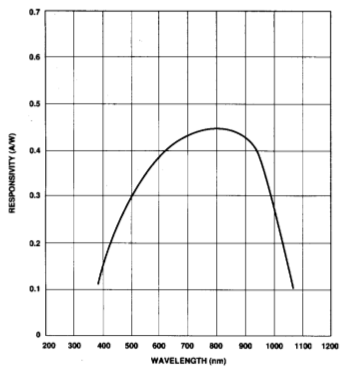
\includegraphics[scale=.45]{responsivity}
\caption{Responsività spettrale di OSD-15}
\label{fig:responsivity}
\end{figure}

Il rivelatore è stato collegato ad un circuito a transimpedenza come mostrato in figura \ref{fig:trans}

\begin{figure}[htp]
\centering
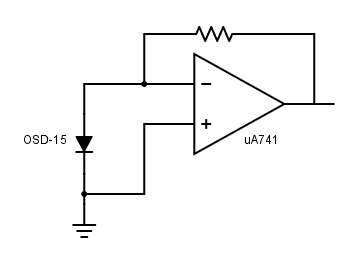
\includegraphics[scale=.45]{transimpedance}
\caption{Circuito a transimpedenza collegato al rivelatore}
\label{fig:trans}
\end{figure}

Come resistenza di feedback è stata scelta R = 55.6(4) $\Omega$.

Il laser impegato è un modello %nome modellooooo
con lunghezza d'onda di 779 nm, che cade quindi intorno al massimo di responsività spettrale del rivelatore. È stato collegato ad un circuito di controllo
%nome circuito
come mostrato in figura \ref{fig:laser}.

\begin{figure}[htp]
\centering
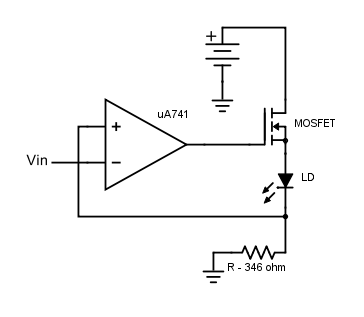
\includegraphics[scale=.5]{laser}
\caption{Circuito di controllo per il laser}
\label{fig:laser}
\end{figure} 

Date la corrente di soglia e la potenza emessa dal laser ad un altro valore di corrente maggiore di quello di soglia è facile determinare il valore della tensione $V_{in}$ perché il laser emetta la potenza desiderata. Infatti se $I_{thr}$ è la corrente di soglia, $I_f$ e $W_f$ un altro valore di corrente,con $I>I_{thr}$, e la relativa potenza, dal momento che la curva W-I per correnti superiori alla soglia è praticamente lineare, si può scrivere in questo regime:
\begin{equation}
W(I) = W_f \frac{I-I_{thr}}{I_f - I_{thr}}
\end{equation}

Dalle regole d'oro degli op-amp si ha che, facendo riferimento al circuito di figura \ref{fig:laser}:

\begin{equation}
I = \frac{V_{in}}{R}
\end{equation}

da cui è possibile ricavare sia la corrente che deve scorrere nel laser per ottenere una data potenza sia la tensione in ingresso per generare quella corrente. Ad esempio per ottenere 0.1 mW di potenza se $I_{thr} = 17\, mA$, $I_f = 25 \, mA$ e $W_f= 2.2 \, mW$ si ha:
\begin{gather}
I = 17.36 \, mA \\
V_{in} = 17.36 \, R
\end{gather}

dove R è in ohm e $V_{in}$ in mV. Nel nostro caso non avendo avuto a disposizione un valore affidabile per applicare le relazioni precedenti abbiamo dovuto determinare direttamente, tramite un rivelatore di potenza incidente portatile,
%nome del coso usato da di lieto
la tensione in ingresso all'op-amp per ottenere una potenza emessa di 0.3 mW, risultando essere di 6.54 V. Il valore della resistenza di carico impiegata è R = (346 $\pm$ 3) $\Omega$.\\
Le misure in questa fase sono state effettuate tramite il VI \texttt{Vin$\_$Vout$\_$2C}, che permette di impostare sia la tensione in uscita ad un canale di output della scheda DAQ, nel nostro caso la CB22, che di rilevare le tensioni in due canali. Abbiamo quindi collegato la CB22 all'ingresso dell'opamp del circuito di controllo del laser e rilevato la tensione in uscita all'opamp collegato al rivelatore. Per le regole d'oro dell'op-amp, quest'ultima tensione è anche la d.d.p. ai capi della resistenza di feedback. È così possibile determinare direttamente la corrente generata dal rivelatore è tramite la responsività spettrale, che a 780 nm vale circa 0.45 A/W, la potenza incidente sul rivelatore.\\
Il laser e il rivelatore sono stati inseriti entro due fessure speculari di un supporto al cui interno è possibile incastrare le cuvette per le misure di assorbimento. La prima misura, effettuata a "vuoto", ha fornito $V_{out} = 3.70(5) V$ che per quanto detto in precedenza corrisponde ad una potenza incidente di 0.150(3) mW, la metà di quella che dovrebbe essere generata dal laser. Il motivo per cui si ottiene la metà di quello previsto potrebbe essere dovuto alla non perfetta collinearità del fascio laser e al fatto che non tutta la superficie del rivelatore è utile alla ricezione della radiazione.\\
La misura è stata ripetuta inserendo una cuvette vuota, effettuando le rilevazioni più volte inserendo più volte la cuvette, sia dal lato chiaro che opaco. I risultati sono riassunti in tabella \ref{tab:empty}.

\begin{table}[htp]
\centering
\caption{Misure con cuvette vuota}
\label{tab:empty}
\begin{tabular}{c|c}
\textbf{Lato chiaro} & 3.617(1) V ~ 0.1446(1) mW \\ 
\hline 
\textbf{Lato oscuro} & 3.408(1) V ~ 0.1362(1) mW \\ 
\end{tabular} 
\end{table}

Al ripetere delle misure il valore è rimasto stabile, le uniche variazioni rilevate nell'ultima cifra significativa dei risultati riportati sempre in tabella \ref{tab:empty}.

\subsection{Misure di assorbimento}

Per le misure di assorbimento si aveva a dispsizione delle cuvette con soluzioni di CuSO$_4$ in diverse concentrazioni. Le cuvette sono state inserite fra laser e rivelatore tramite l'apposito supporto ed è stata misurata la tensione all'uscita del'opamp nel circuito di figura \ref{fig:trans}, da cui come si è visto è possibile determinare la potenza incidente sul rivelatore. Nell'effettuare le misure le cuvette sono state posizionate più volte per verificare la ripetività della misura stessa. Abbiamo misurato l'assorbimento sia quando il laser incideva sui lati trasparenti che opachi delle cuvette. Riportiamo in tabella \ref{tab:001} i dati grezzi relativi al caso 0.01 M.

\begin{table}[htp]
\centering
\caption{Dati relativi al caso 0.01 M}
\label{tab:001}
\begin{tabular}{c|c}
\hline \textbf{Lato Chiaro} &\textbf{ Lato Oscuro} \\ 
\hline 
3.494 & 3.228 \\ 
\hline 
3.514 & 3.293 \\ 
 
3.511 & 3.247 \\ 
 
3.501 & 3.271 \\ 

3.491 & 3.193 \\ 
 
3.501 & 3.232 \\ 
 
3.478 & / \\		 

3.472 & / \\	 
 
3.457 & / \\ 
\hline
\end{tabular} 
\end{table}

Sono stati raccolti prima i primi 6 dati lato trasparente, poi quelli lato opaco e infine gli ultimi 3 lato trasparente. Si nota come la tensione registrata per questi ultimi dati sia significativamente diversa dai primi 6 dati, per di più lo stesso fenomeno è stato osservato anche per altre cuvette, cioè tensioni sensibilmente inferiori dopo aver fatto la misura con il lato opaco. È possibile che all'interno della stessa serie di misure (senza passare da un lato all'altro) involontariamente non si è spostato molto il punto in cui la radiazione laser incide sulla parete, mentre cambiando lato della cuvette si è ''persa memoria'' della posizione precedente rilevando così delle disomogeneità nella costituzione delle pareti. In ogni caso si è verificato che l'errore si mantenesse entro l' 1 $\%$.\\
Sono state infine effettuate le misure al variare della concentrazione, mediando sui diversi posizionamenti delle cuvette. In tabella \ref{tab:att} sono riportati i dati di $\frac{I}{I_0}$ in funzione della molarità, dove per $I_0$ sono stati presi i due valori di tabella \ref{tab:empty}, mentre un plot dei dati è mostrato in figura \ref{fig:att}.

\begin{table}[htp]
\centering
\caption{Attenuazioni in funzione della molarità}
\label{tab:att}
\begin{tabular}{c|c|c}
\hline 
\textbf{Lato Chiaro} & \textbf{Lato oscuro} & \textbf{Molarità (mol)}\\ 	
\hline 
0.964(1) & 0.952(3) & 0.01 \\ 

0.932(1) & 0.912(3) & 0.025 \\ 

0.659(3) & 0.521(2) & 0.04 \\ 

0.504(1) & 0.3590(6) & 0.06 \\ 

0.211(1) & 0.1487(6) & 0.1 \\ 

0.0280(5) & 0.0218(1) & 0.15 \\ 

0.00083(5) & 0.00085(5) & 0.25 \\ 

0.00077(5) & 0.00082(5) & 0.4 \\ 

0.00071(1) & 0.00075(1) & 1 \\ 

0.00071(1) & 0.00075(1) & 1.2 \\
\hline  
\end{tabular} 
\end{table}

\begin{figure}[htp]
\centering
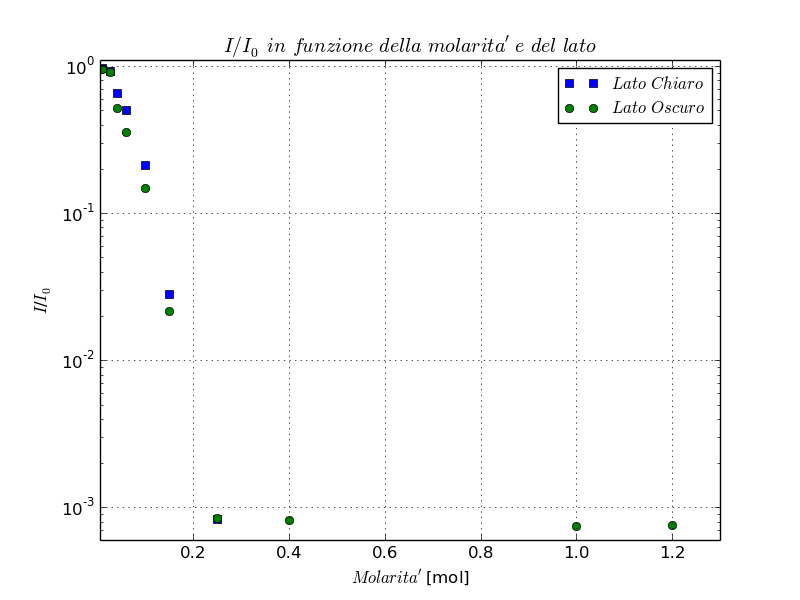
\includegraphics[scale=.6]{plotpowerrel}
\caption{Plot attenuazione in funzione della molarità}
\label{fig:att}
\end{figure}

Come si vede, per alte molarità l'attenuazione non segue un'andamento esponenziale, ma si mantiene approssimativamente costante. Questo potrebbe essere dovuto al fatto che a queste concentrazioni possono cadere alcune ipotesi su cui si basa la legge di Beer-Lambert, in particolare quella di centri assorbenti indipendenti. Per M = 0.01 si ha anche un significativo discostamento dall'andamento lineare dei dati centrali. Una possibile spiegazione in questo caso potrebbe essere che altre cause di attenuazione prevalgono rispetto a quelle dovute all'assorbimento da parte di CuSO$_4$, ad esempio la diffusione per scattering dei fotoni sulle molecole d'acqua o le pareti delle cuvette.\\
È stato fatto un fit dei dati relativi al lato chiaro lasciando libero il valore di $I_0$ secondo l'equazione:

\begin{equation}
\frac{I}{I_0}=C e^{- \alpha _u (\lambda) c x}
\end{equation}

tenendo conto dello spessore standard di 1 cm delle cuvette. Sono stati considerati solo i dati nella regione lineare, per cui sono stati esclusi il primo e gli ultimi tre dati. I risultati sono mostrati in figura \ref{fit:2} e in tabella \ref{tab:fit}.

\begin{figure}[!h]
\centering
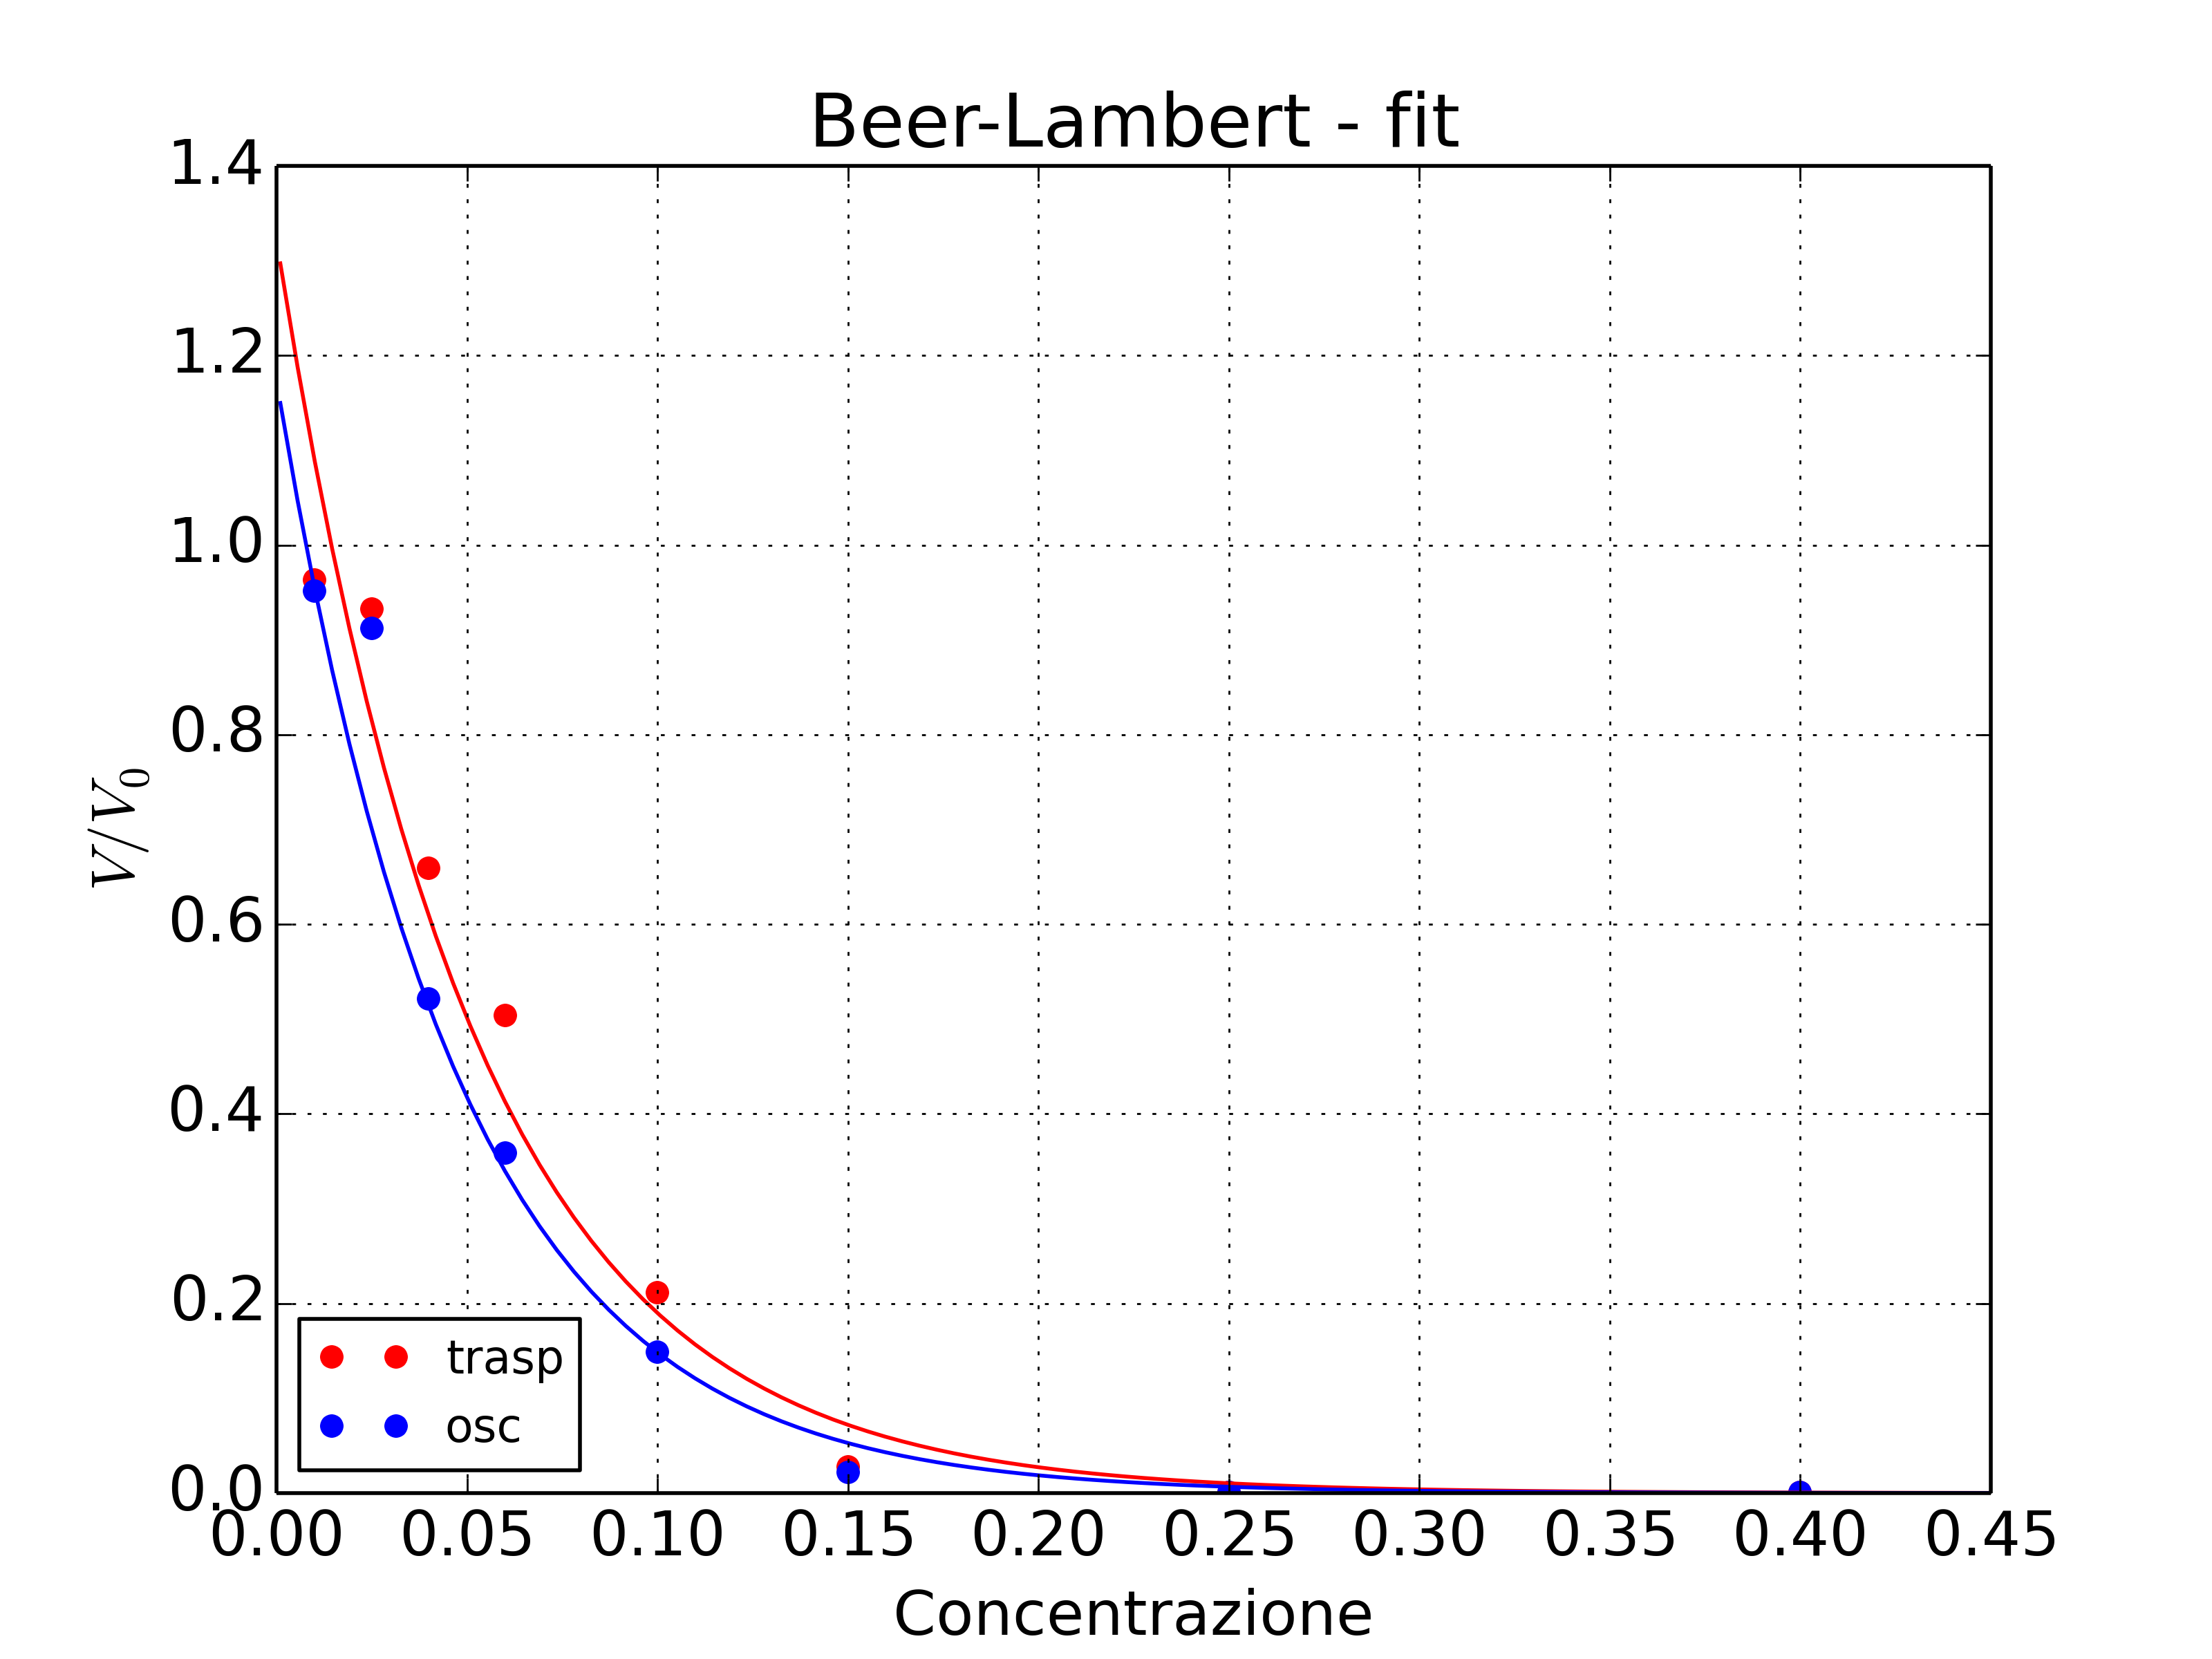
\includegraphics[scale=.6]{./concentr_es5}
\caption{Fit a due parametri dei dati sperimentali}
\label{fit:2}
\end{figure}

\begin{table}[!h]
\centering
\caption{Risultati fit, $\lambda$ = 779 nm}
\label{tab:fit}
\begin{tabular}{c|c|c}
\textbf{Lato} & \textbf{Chiaro} & \textbf{Oscuro} \\
\hline
$\alpha _u (\lambda)$ [cm$^{-1}$ mol$^{-1}$]& 19(2) & 20(2) \\ 
\hline 
C & 1.3(1) & 1.17(4) \\ 
\end{tabular} 
\end{table}

I risultati del fit non sembrano graficamente troppo buoni: in particolare la curva per il lato chiaro non sembra fittare al meglio i dati sperimentali. E' stato provato a fittare linearmente il logaritmo delle tensioni ma i risultati dei parametri non cambiano sostanzialmente. Possiamo comunque notare come i valori del coefficiente di assorbimento nei due casi sia venuto identico, cosa che effettivamente ci aspettava dal momento che normalizzando con l'assorbimento delle cuvette vuote si dovrebbe essere eliminata una differenza fra i due lati. Il coefficiente \emph{C} risulta prossimo ad 1, quindi sembrerebbe che il contributo dell'acqua all'attenuazione della radiazione incidente sia molto piccolo ma comunque evidente.\\

Eseguiamo adesso le stesse misure di assorbanza per diverse potenze del laser e con concentrazioni inferiori a 0.25M, per le quali si è visto circa rispettato l'andamento esponenziale di Beer-Lambert. Le potenze scelte per il laser sono circa 0.540mW, 0.680mW e 0.750mW, corrispondenti a tensioni di ingresso nel circuito di controllo di 7.20V, 7.60V e 7.80V. Per ognuna di queste potenze si sono effettuate misurazioni sia per il lato trasparente che per quello opaco. Nel plot in Figura (\ref{es9_concentrazioni}) sono riportati i dati sperimentali acquisiti per tutte e tre le tensioni, sia in scala lineare che in scala semilogaritmica (le tensioni in uscita sono state normalizzate a 1 in base a quella misurata con la cuvette vuota, in modo da avere un'intensità percentuale residua). \\



\begin{figure}
\centering
\subfloat[Subfigure 1 list of figures text][Dati sprimentali scala lineare.]{
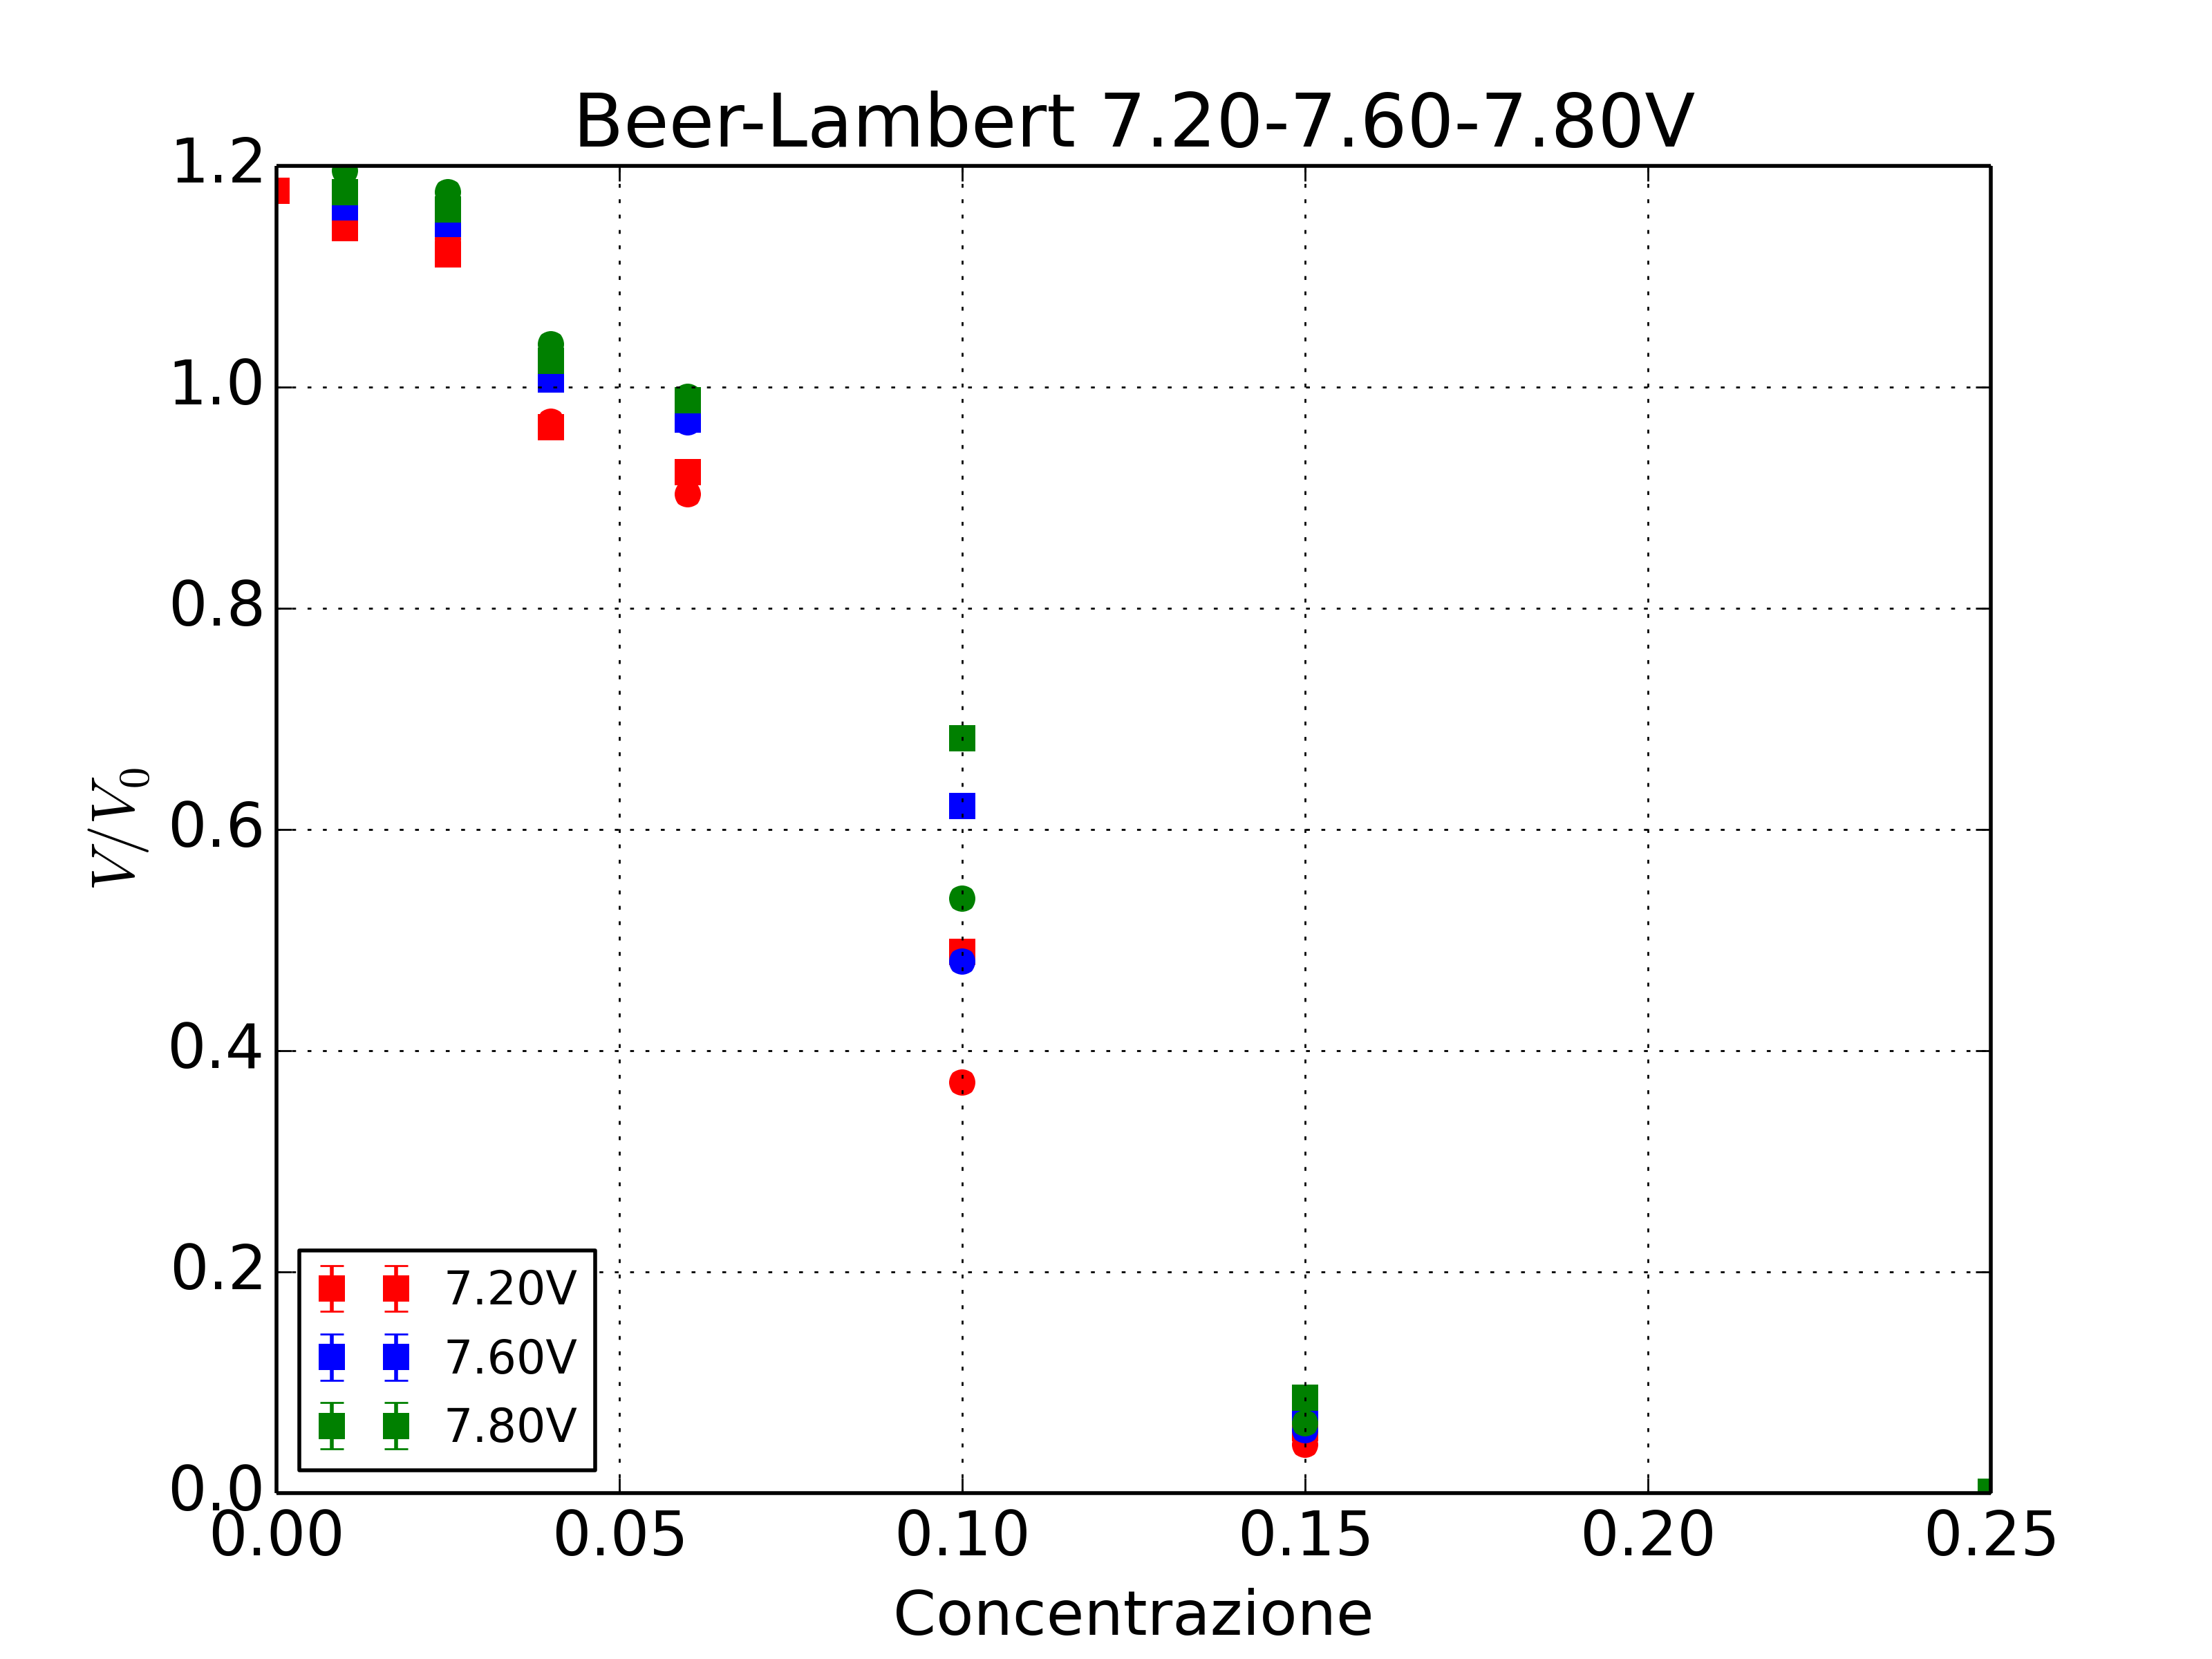
\includegraphics[width=0.5\linewidth]{./es9_concentr}
\label{fig:es9_concentr}}
%\qquad
\subfloat[Subfigure 2 list of figures text][Dati sperimentali scala logaritmica.]{
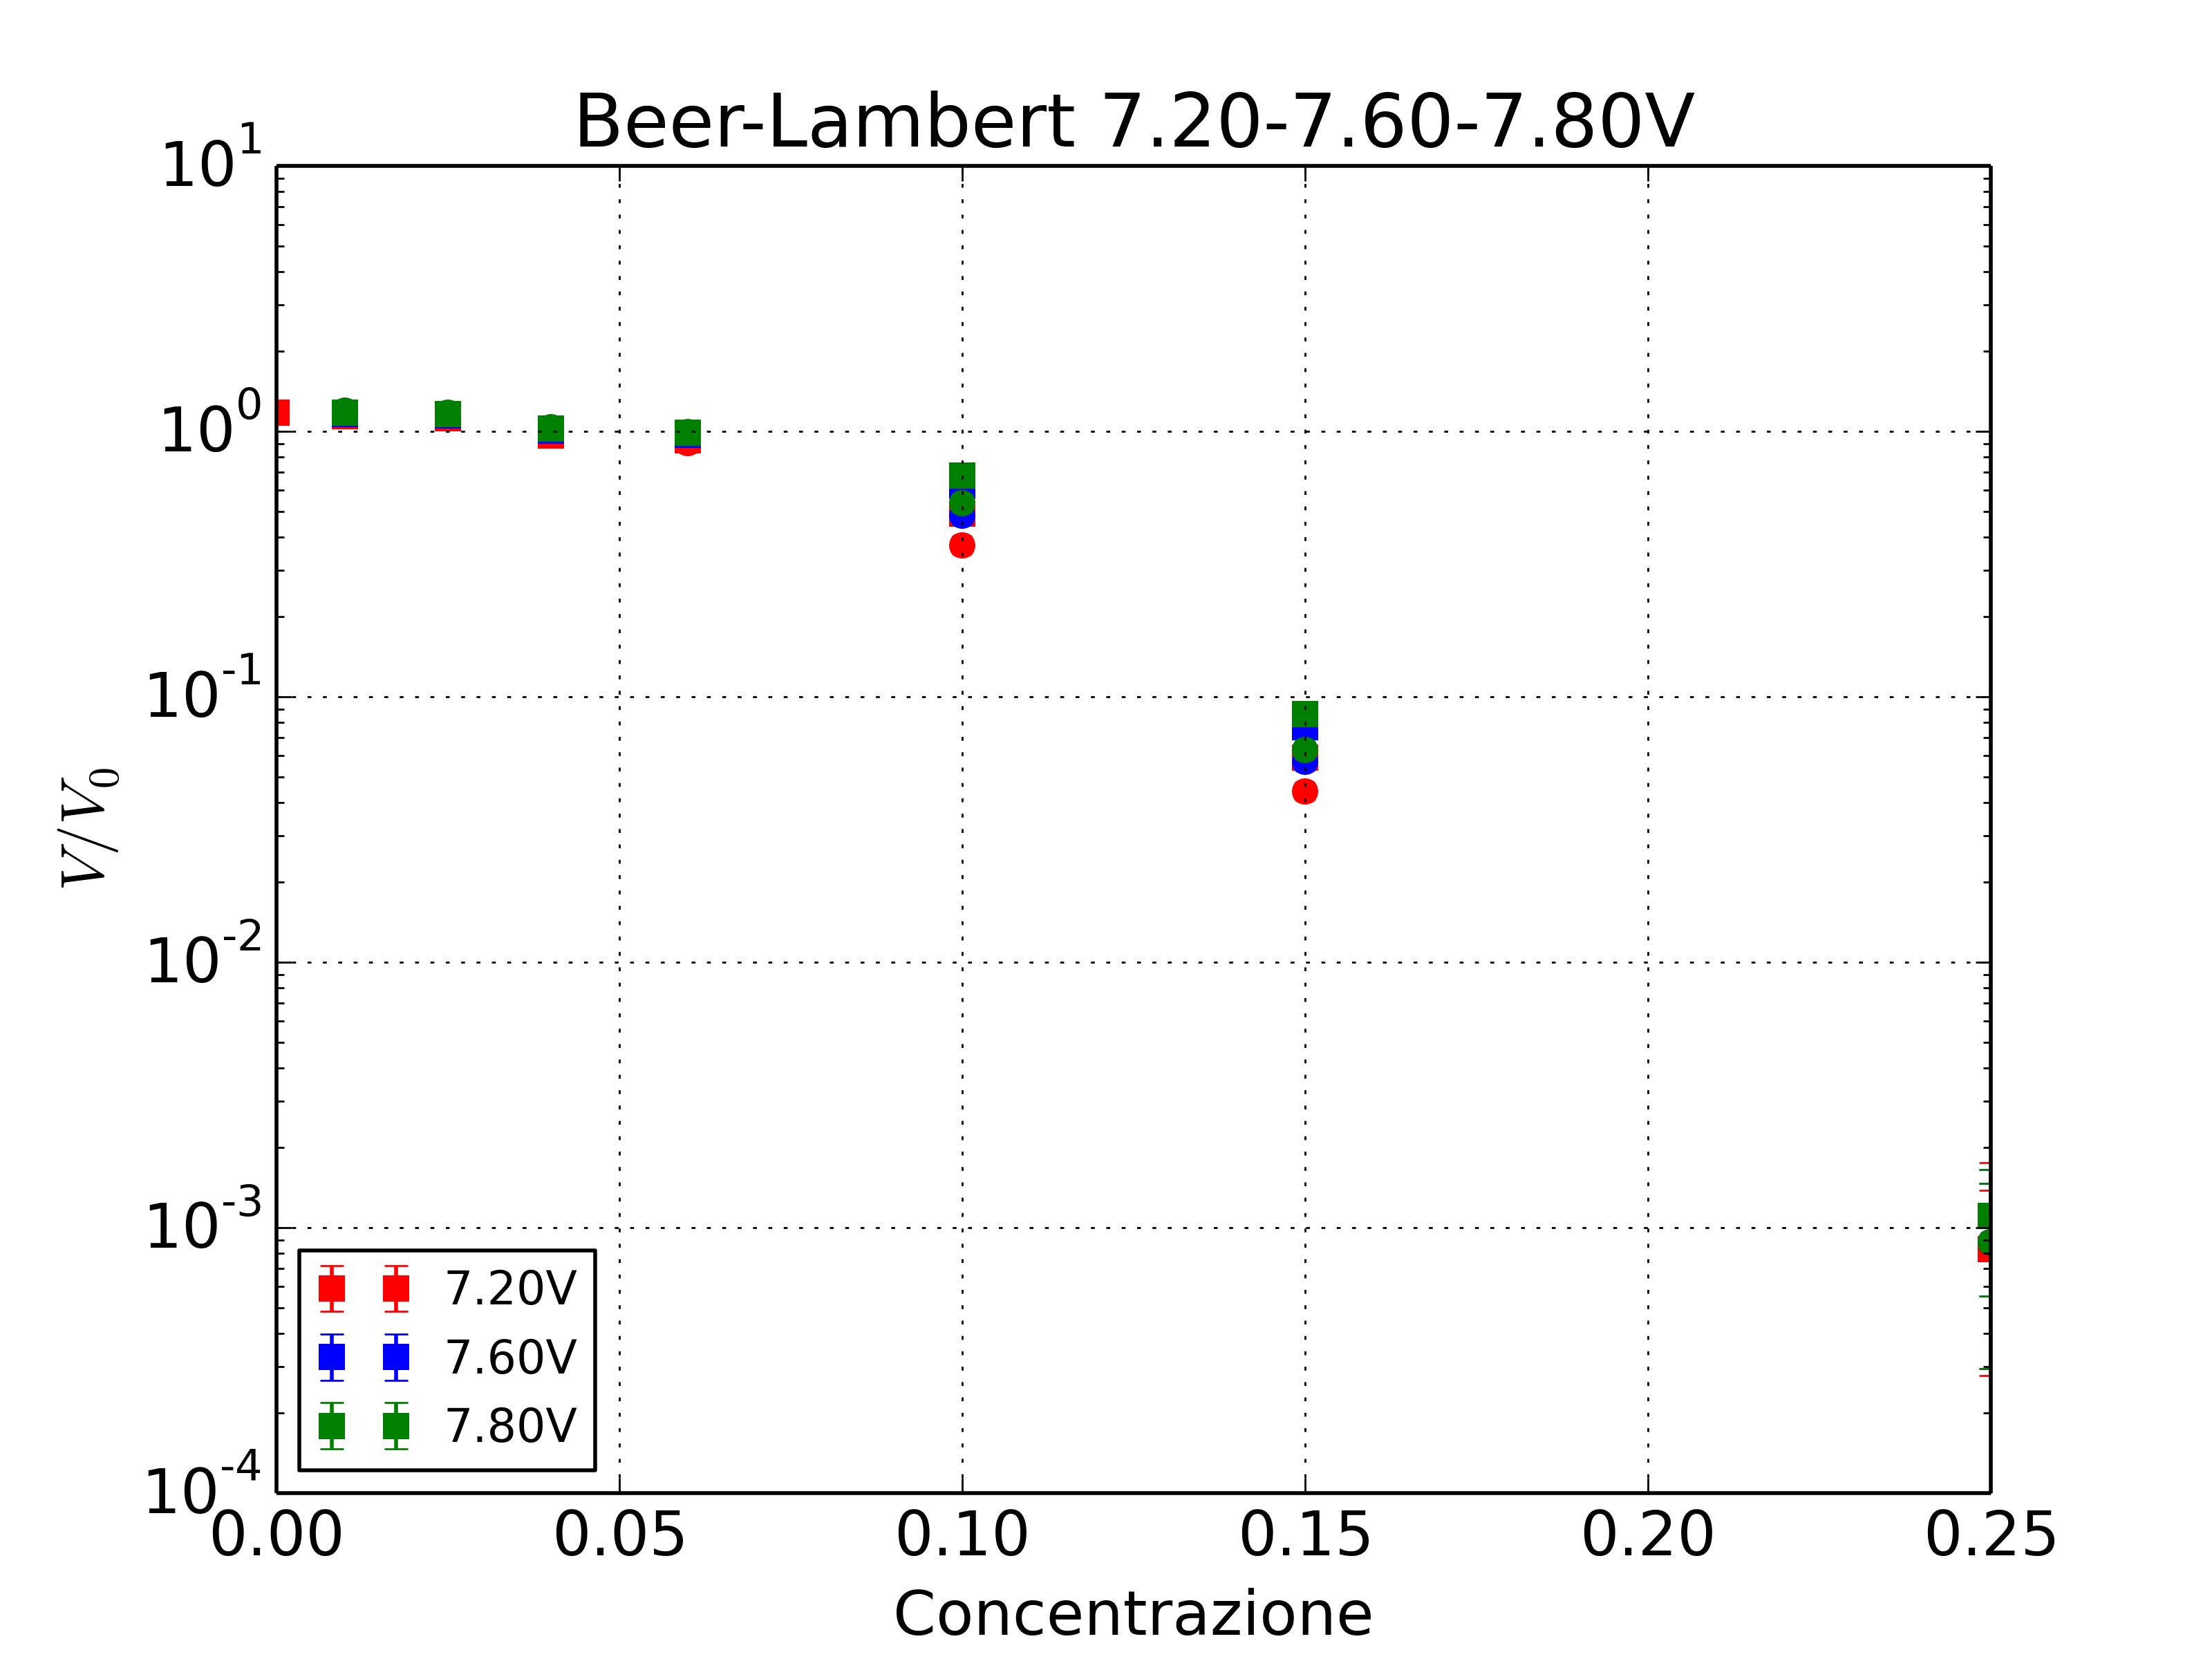
\includegraphics[width=0.5\linewidth]{./es9_concentr_semilogy}
\label{fig:es9_concentr_semilogy}}
%\qquad

\caption{Plot delle assorbanze: con i quadratini sono rappresentate le acquisizioni per il lato trasparente, con i pallini quelle dal lato oscuro.}
\label{es9_concentrazioni}
\end{figure}

L'andamento esponenziale non sembra bellissimo, ma possiamo comunque provare a fittare la legge di Beer Lambert per ciascuna curva (sono 6). I risultati sono riportati nella tabella di seguito e un esempio per la tensione 7.20V è in Figura (\ref{fig:concentr_7_20_fit}).

\begin{table}[h]
\centering
\begin{tabular}{c|c|c|c|c|c|c}
  & \textbf{7.20}V (tr) & \textbf{7.20V} (op)  & \textbf{7.60V} (tr) & \textbf{7.60V} (op) & \textbf{7.80V} (tr) & \textbf{7.80V} (op)\\ 
\hline Assorbanza & 11.4(2.4) & 13.9(2.2) & 11.4(2.2) & 12.7(2.2) & 11.0(2.2) & 12.3(2.2) \\ 
 C & 1.3(0.1) & 1.5(0.2) & 1.5(0.2) & 1.5(0.2) & 1.5(0.2) & 1.5(0.2)\\ 
\hline
\end{tabular} 
\end{table}


\begin{figure}
\centering
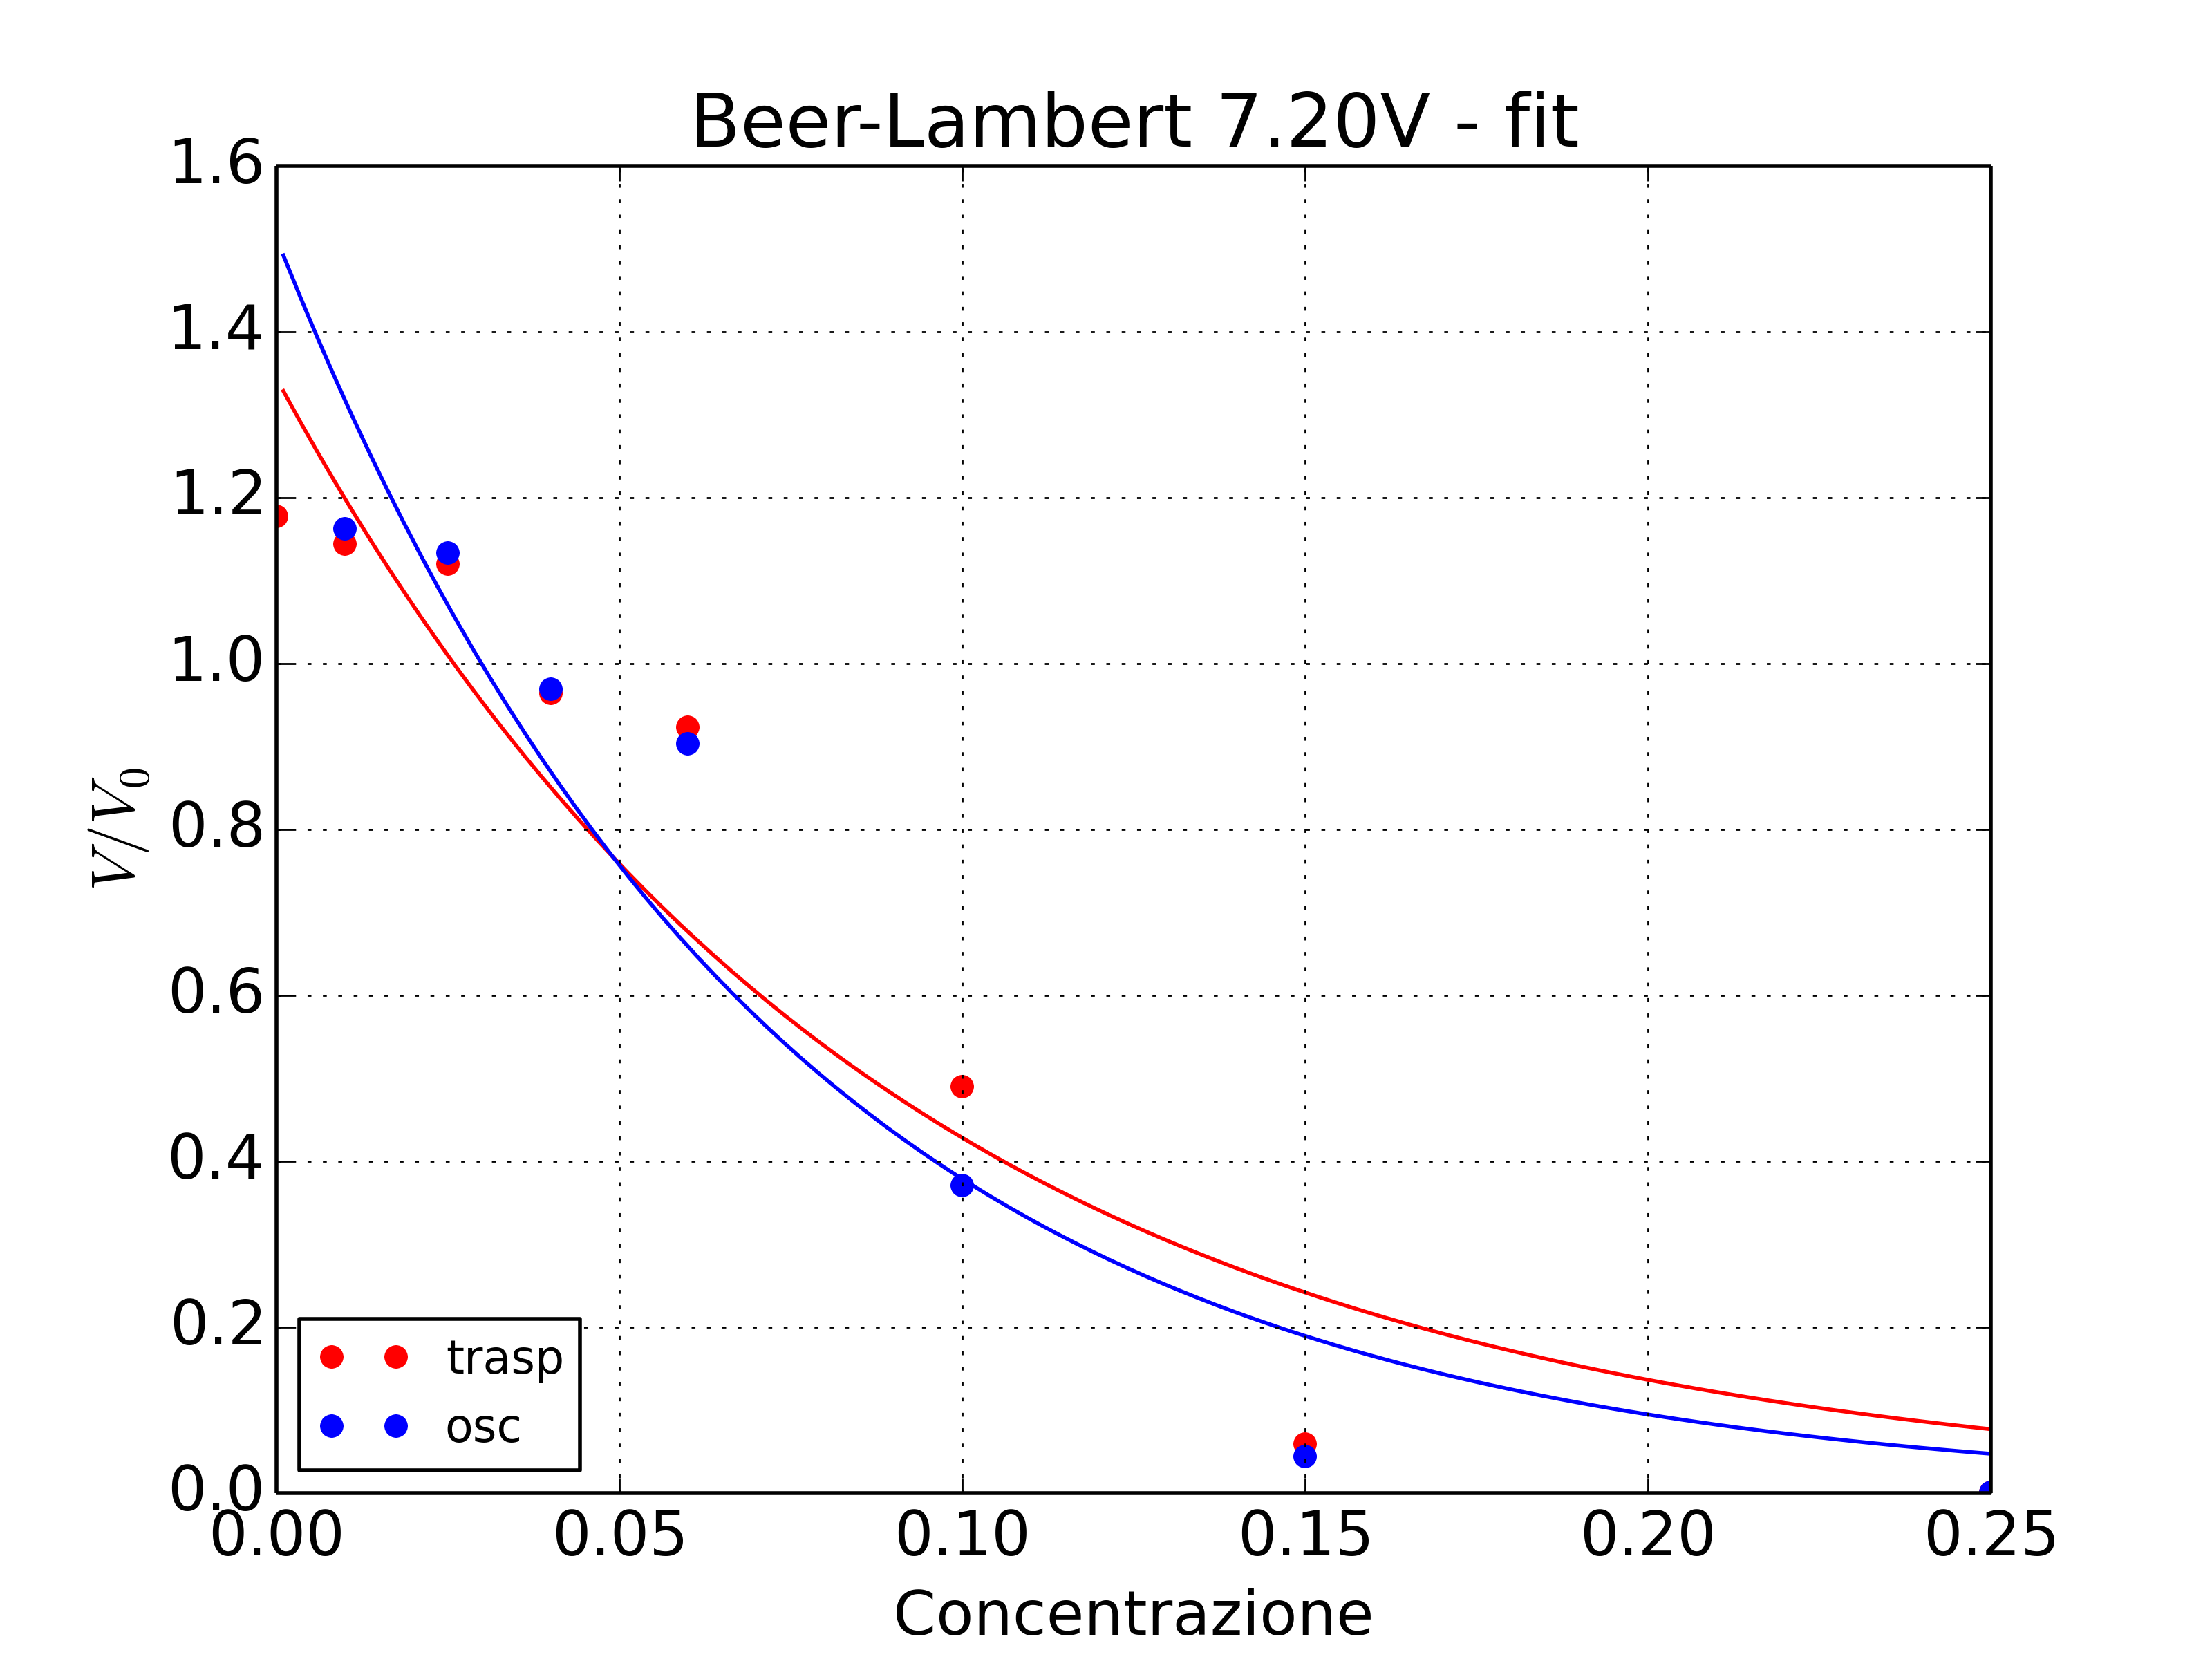
\includegraphics[width=0.7\linewidth]{./concentr_7_20_fit}
\caption{Fit di Beer-Lambert per la tensione di 7.20V (540mW)}
\label{fig:concentr_7_20_fit}
\end{figure}

I coefficienti di assorbanza sono tutti piuttosto simili fra di loro e sono compatibili nei limiti dell'errore (che comunque è piuttosto alto, anche il 15 \%). Disturba, invece, la considerevole differenza con i coefficienti ottenuti precedentemente: sembra che la regione di x-y esplorata dal fit induca un cattivo condizionamento del programma di fit tale che, variando di poco la disposizione dei punti, i risultati siano molto diversi. Non solo, anche l'assegnazione degli errori sembra giocare un ruolo rilevantissimo nel risultato della routine di fit, cosa che ci lascia qualche perplessità sulla validità dei risultati.\\
Tuttavia, almeno in questo caso, possiamo fare una cosa più furba: il coefficiente di assorbanza dipende dalla sezione d'urto del fascio incidente sui centri di scattering, che a sua volta dipende dall'energia del fascio ma non dal flusso di quest'ultimo (infatti la definizione di sezione d'urto come Rate di reazione/corrente incidente la rende indipendente da questo parametro). Quando noi aumentiamo la potenza del laser stiamo variando solo il numero di fotoni incidenti per unità di volume, e non la loro energia, poichè il laser oltretutto ha una lunghezza d'onda fissata a 779nm. Per questo motivo può essere vantaggioso eseguire un fit globale di tutte le curve assieme, ciascuna di queste con lo \underline{stesso} parametro di assorbanza e invece differente costante C moltiplicativa all'esponenziale (che dipende essenzialmente dalla presenza delle pareti della cuvette). I risultati di questa procedura, che è particolarmente agevole da fare tramite l'uso della routine \textsc{leastsq} di Python, sono di seguito:

\begin{table}[h]
\centering
\begin{tabular}{c|c|c|c|c|c|c}
 & \textbf{7.20}V (tr) & \textbf{7.20V} (op)  & \textbf{7.60V} (tr) & \textbf{7.60V} (op) & \textbf{7.80V} (tr) & \textbf{7.80V} (op)\\ 
\hline Assorbanza & 12.0(0.9) & 12.0(0.9) & 12.0(0.9) & 12.0(0.9) & 12.0(0.9) & 12.0(0.9) \\ 
 C & 1.36(0.09) & 1.4(0.1) & 1.5(0.1) & 1.5(0.1) & 1.5(0.1) & 1.5(0.1)\\ 
\hline
\end{tabular}
\end{table}

Come si può vedere, l'accuratezza del parametro di assorbanza è molto aumentata, il suo errore percentuale ora è circa del 7\%, e in generale anche gli altri parametri C sono più precisi.

\section{Rivelazione di piccoli segnali}
Per concentrazioni piuttosto elevate (per esempio maggiori di 0.6-1 M) il segnale continuo osservato inizia ad essere molto piccolo (ordini d 2-3 mV) e certamente si può pensare che sia anche sporcato da un consistente livello di rumore, generato dai componenti del circuito rivelatore, in particolare l'offset degli ingressi dell'op-amp che per il \textsc{$\mu$ A741CP} tipicamente è compreso fra i valori di 1-7.5 mV, oppure fluttuazioni statistiche termiche.\\
Per stimare il livello di rumore rispetto a quello del segnale di interesse, in generale si definisce il \textit{signal-to-noise ratio} \textsc{SNR}, il rapporto segnale/rumore appunto, dato dalla relazione:

\begin{equation}
\mathrm{SNR} = \frac{S^2}{\sigma_N^2} 
\end{equation}

Dove $S^2$ è la media temporale del quadrato del segnale, fatta su un tempo molto più lungo del periodo:

\begin{equation}
S^2 = \frac{1}{T} \int_{0}^{T}s^2(t)\mathrm{dt}
\end{equation}

e, per un rumore a media nulla, come è solitamente, si ha la particolare proprietà per cui:

\begin{equation}
\sigma_N^2  = \left< (n - \bar{n})^2 \right> = \left< n^2 \right>
\end{equation}

dove, con $n^2$ si è indicato il quadrato del \textit{noise}.\\
Per segnali costanti nel tempo, è facile risalire all'ampiezza di quest'ultimo mediando $s+n$ nel tempo, dato che abbiamo detto che il rumore ha media nulla. Se, invece, anche il segnale da estrarre varia in funzione del tempo, la procedura è meno immediata. Si possono, tuttavia, ottenere degli ottimi risultati se si conosce la frequenza di tale segnale adottando dei metodi di \textit{lock-in} molto efficienti. In questa sezione verrà introdotta una modulazione periodica, sinusoidale sul livello continuo di tensione fornita al laser, e si cercherà di estrarre con varie tecniche informazioni sulla modulazione, anche in presenza di forti rumori.

\subsection{Modulazione del segnale}
Come si è già detto, il primo passo consiste nell'introdurre una modulazione in tensione, sommandola al livello che stiamo già fornendo al laser. Per farlo, usiamo un circuito sommatore composto da un op-amp impiegato in modalità invertente,al cui ingresso \textsc{IN}- diamo sia la tensione prodotta dalla \textsc{CB22} che quella alternata dal generatore di segnali \textsc{atf10b}, di modo che in uscita avremo la somma delle due. Lo schema del sommatore è riportato in Figura (\ref{fig:sommatore}). Da notare che, essendo l'op-amp impiegato in modalità invertente, la tensione in uscita è chiaramente di segno opposto rispetto a quelle in ingresso; in questo caso vale la formula:

\begin{equation}
V_{out} = - \frac{R_{SOM}}{R_3}V_{ATF} - \frac{R_{SOM}}{R_4}V_{CB22}
\end{equation}   

per cui facciamo attenzione a dare in uscita dalla \textsc{cb22} una tensione negativa. In aggiunta a ciò, poichè è conveniente lavorare alla stessa potenza del laser usata fino ad ora (P $\eqsim$ 0.3mW ), è opportuno usare una modulazione di ampiezza picco-picco $V_{PP} = 100 \mathrm{mV}$, in modo da non cambiare eccessivamente il punto di lavoro e rimanere nei range di tensione di funzionamento del laser. La frequenza della modulazione è stata settata a 300Hz.\\
Le resistenze scelte per il sommatore sono:\\

\begin{table}[h]
\centering
\begin{tabular}{c|c|c}
\hline $R_{SOM}$ & $R_4$ & $R_3$ \\ 
\hline 9.86(1) k$\Omega$ & 10.0(1) k$\Omega$ & 10.05(1) k$\Omega$ \\ 
\end{tabular}
\end{table}  

\begin{figure}
\centering
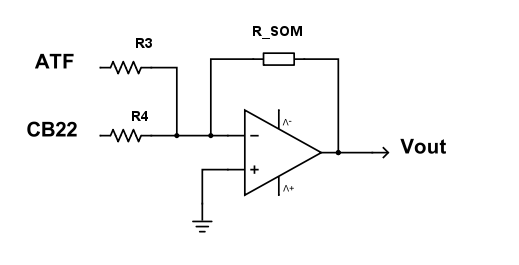
\includegraphics[width=0.7\linewidth]{./sommatore}
\caption{Circuito sommatore del segnale modulato e il fondo continuo.}
\label{fig:sommatore}
\end{figure}


Mandando una tensione $V_{CB22} = -6.67$V il circuito sommatore funziona correttamente e le tensioni sul laser sono nei limiti previsti, per cui possiamo collegare nuovamente la parte di rivelazione con il fotorivelatore. Nel grafico in Figura (\ref{fig:es11_plot}) sono riportati sia la tensione in uscita dal circuito sommatore che quella rilevata dal circuito amplificatore del fotodiodo senza couvette interposta: si nota la frequenza uguale per i due segnali (ovviamente) e la presenza in entrambi i casi della modulazione. Il valore picco-picco stimato di quest'ultima (nel circuito rivelatore) è di circa 60mV, a fronte dei circa 100mV in uscita dal sommatore.\\

\begin{figure}
\centering
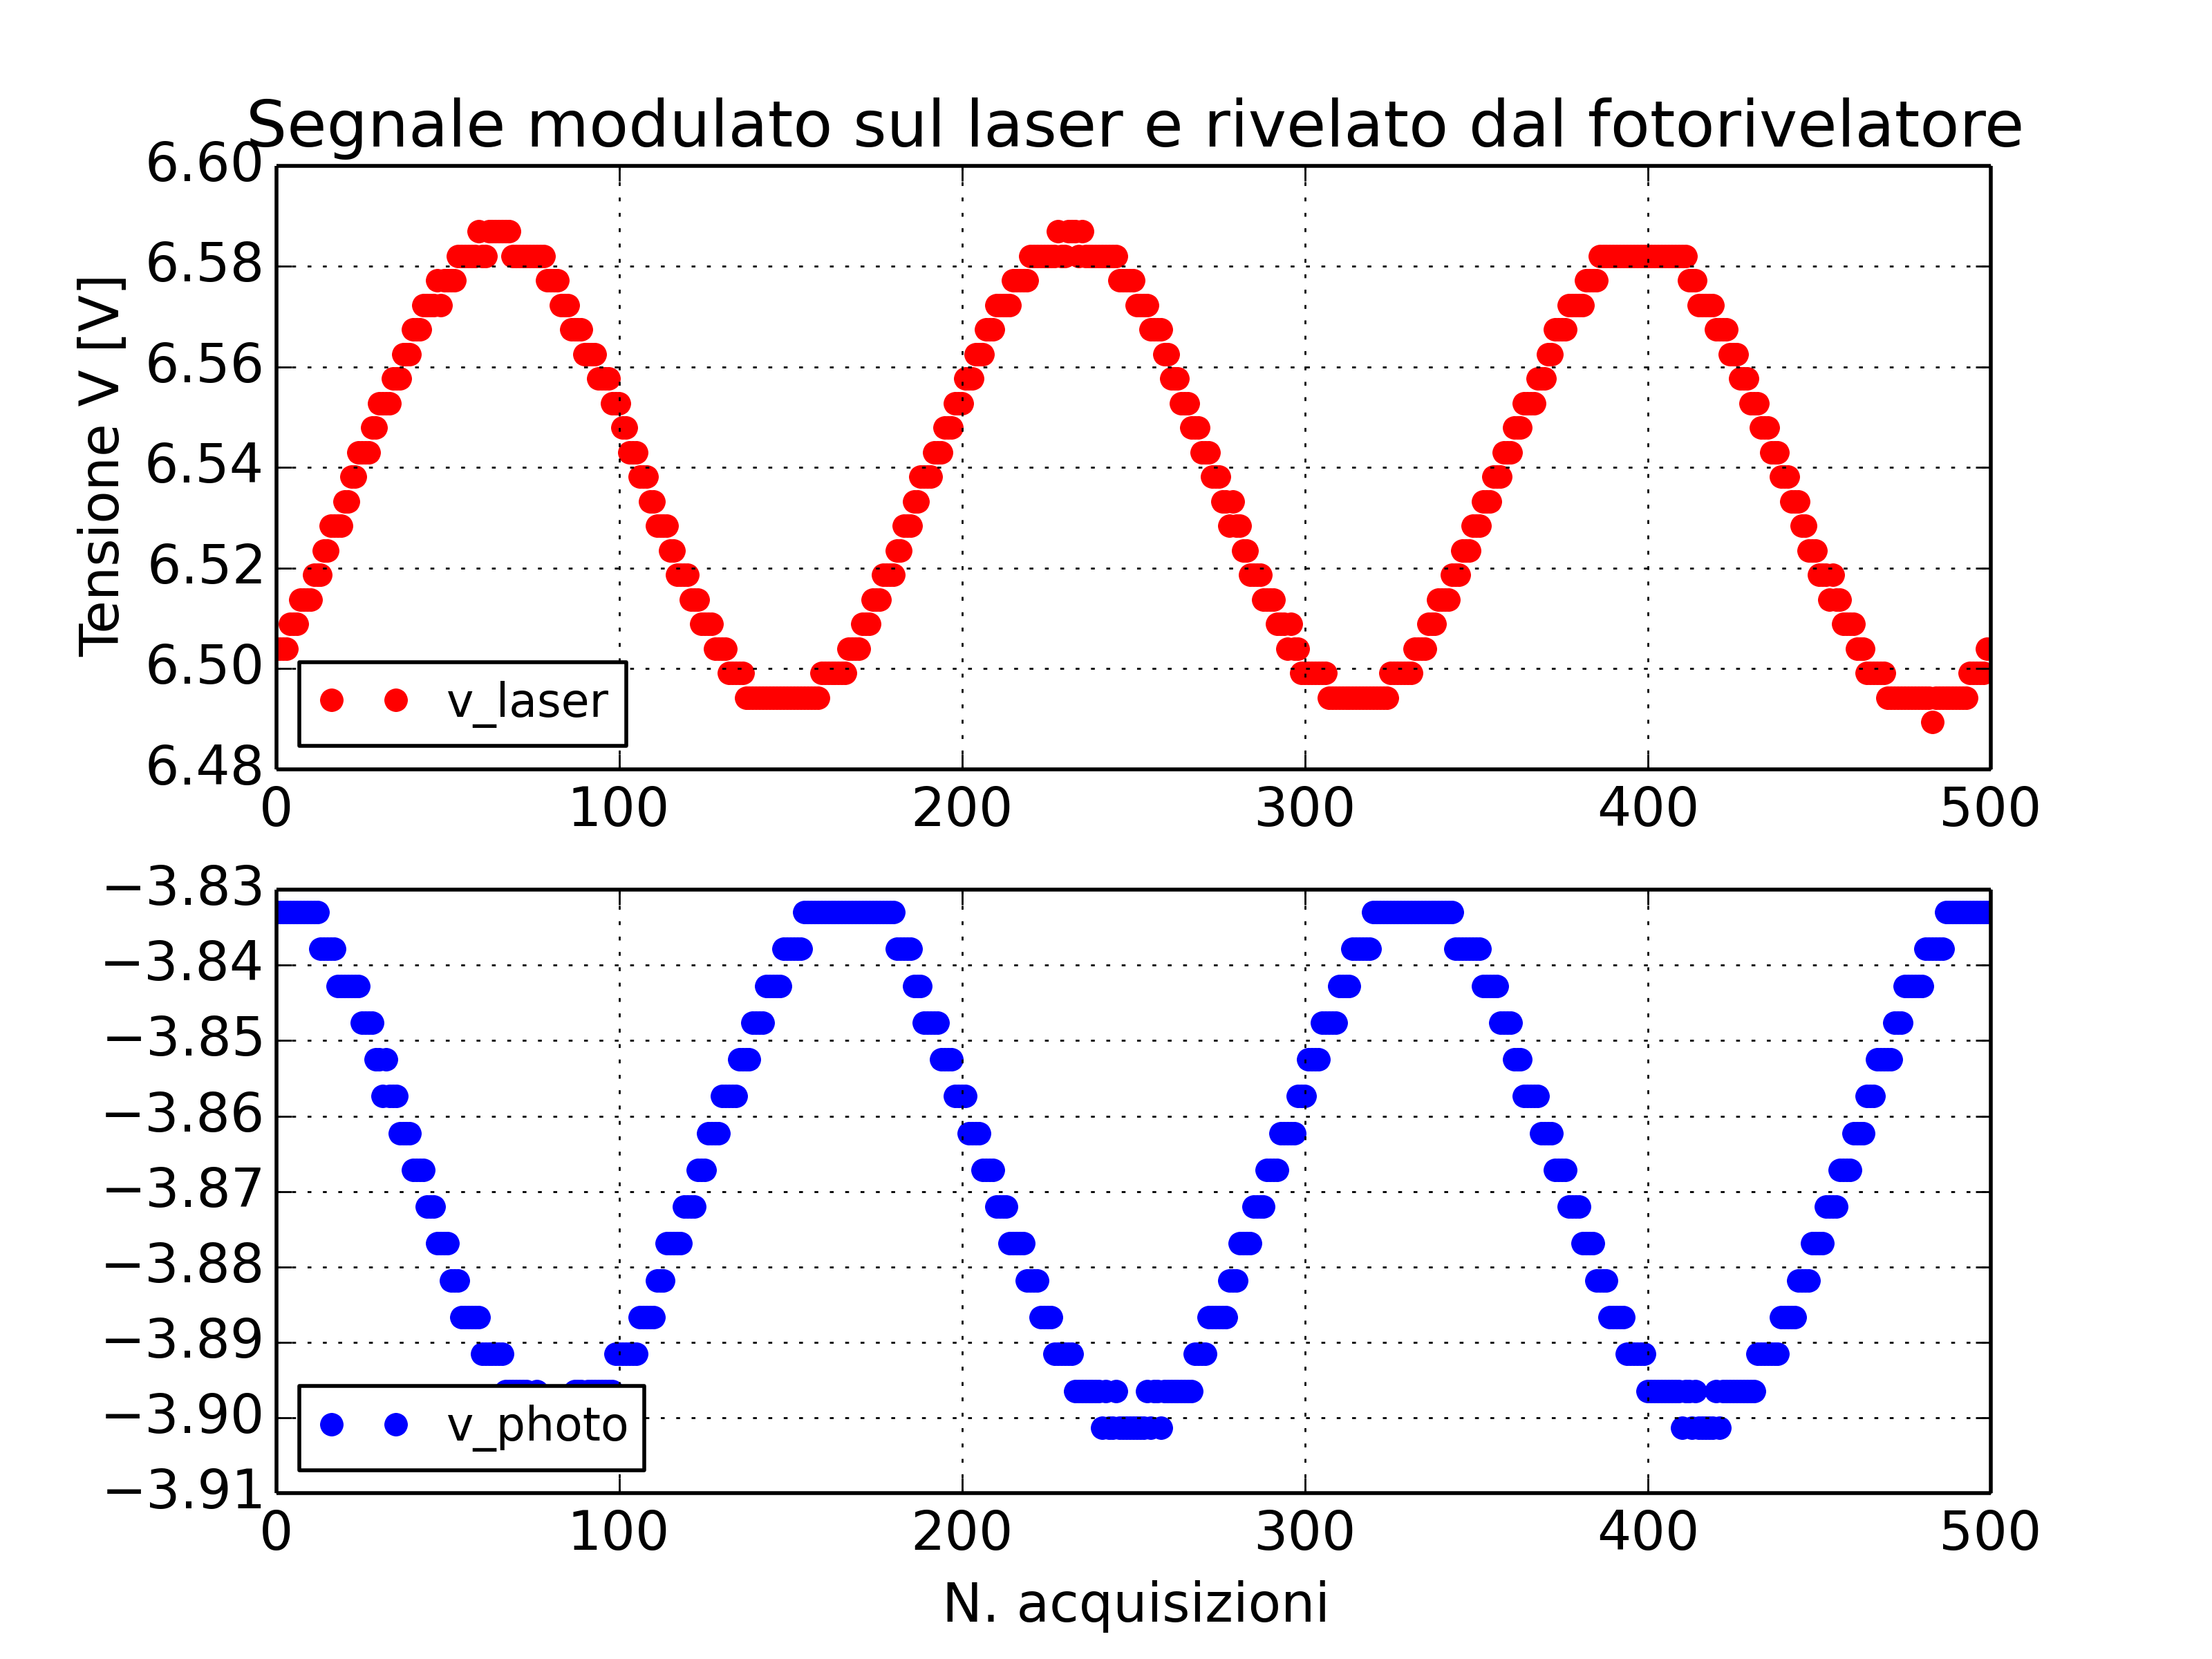
\includegraphics[width=0.8\linewidth]{./es11_plot}
\caption{Modulazione sul laser e sul fotorivelatore}
\label{fig:es11_plot}
\end{figure}


Possiamo a questo punto ripetere la stessa serie di misurazioni per varie concentrazioni di soluzione, segnando ogni volta la differenza picco-picco e provando a fittare una esponenziale come nella ( \%numero eq. beer-lambert). Purtroppo, bisogna segnalare un'imprevista difficoltà dovuta al probabile (certo) scambio di alcune cuvette nel supporto fra le diverse concentrazioni. Infatti, durante l'acquisizione stessa dei dati $V_{PP}$ si sono notate evidenti incongruenze poichè con concentrazioni maggiori si aveva un segnale più alto di quello di concentrazioni \textit{supposte} minori. Provando a permutare alcuni valori fra le diverse concentrazioni possibili è stato possibile fittare un'assorbanza simile a quella ottenuta nella sezione precedente, da prendere comunque con il beneficio del dubbio. Di seguito si riportano le tensioni $V_{PP}$ per ogni concentrazione molare e in Figura (\ref{fig:es13_tens_piccopicco_plot_mod}) i risultati del fit.\\

\begin{table}[h]
\centering
\begin{tabular}{c|c}
Assorbanza [$\mathrm{cm}^{-1}\mathrm{mol}^{-1}$] &  C [V] \\ 
\hline 13.8(8) & 0.264(7) \\ 
 
\end{tabular} 
\end{table}
~\\


\begin{figure}
\centering
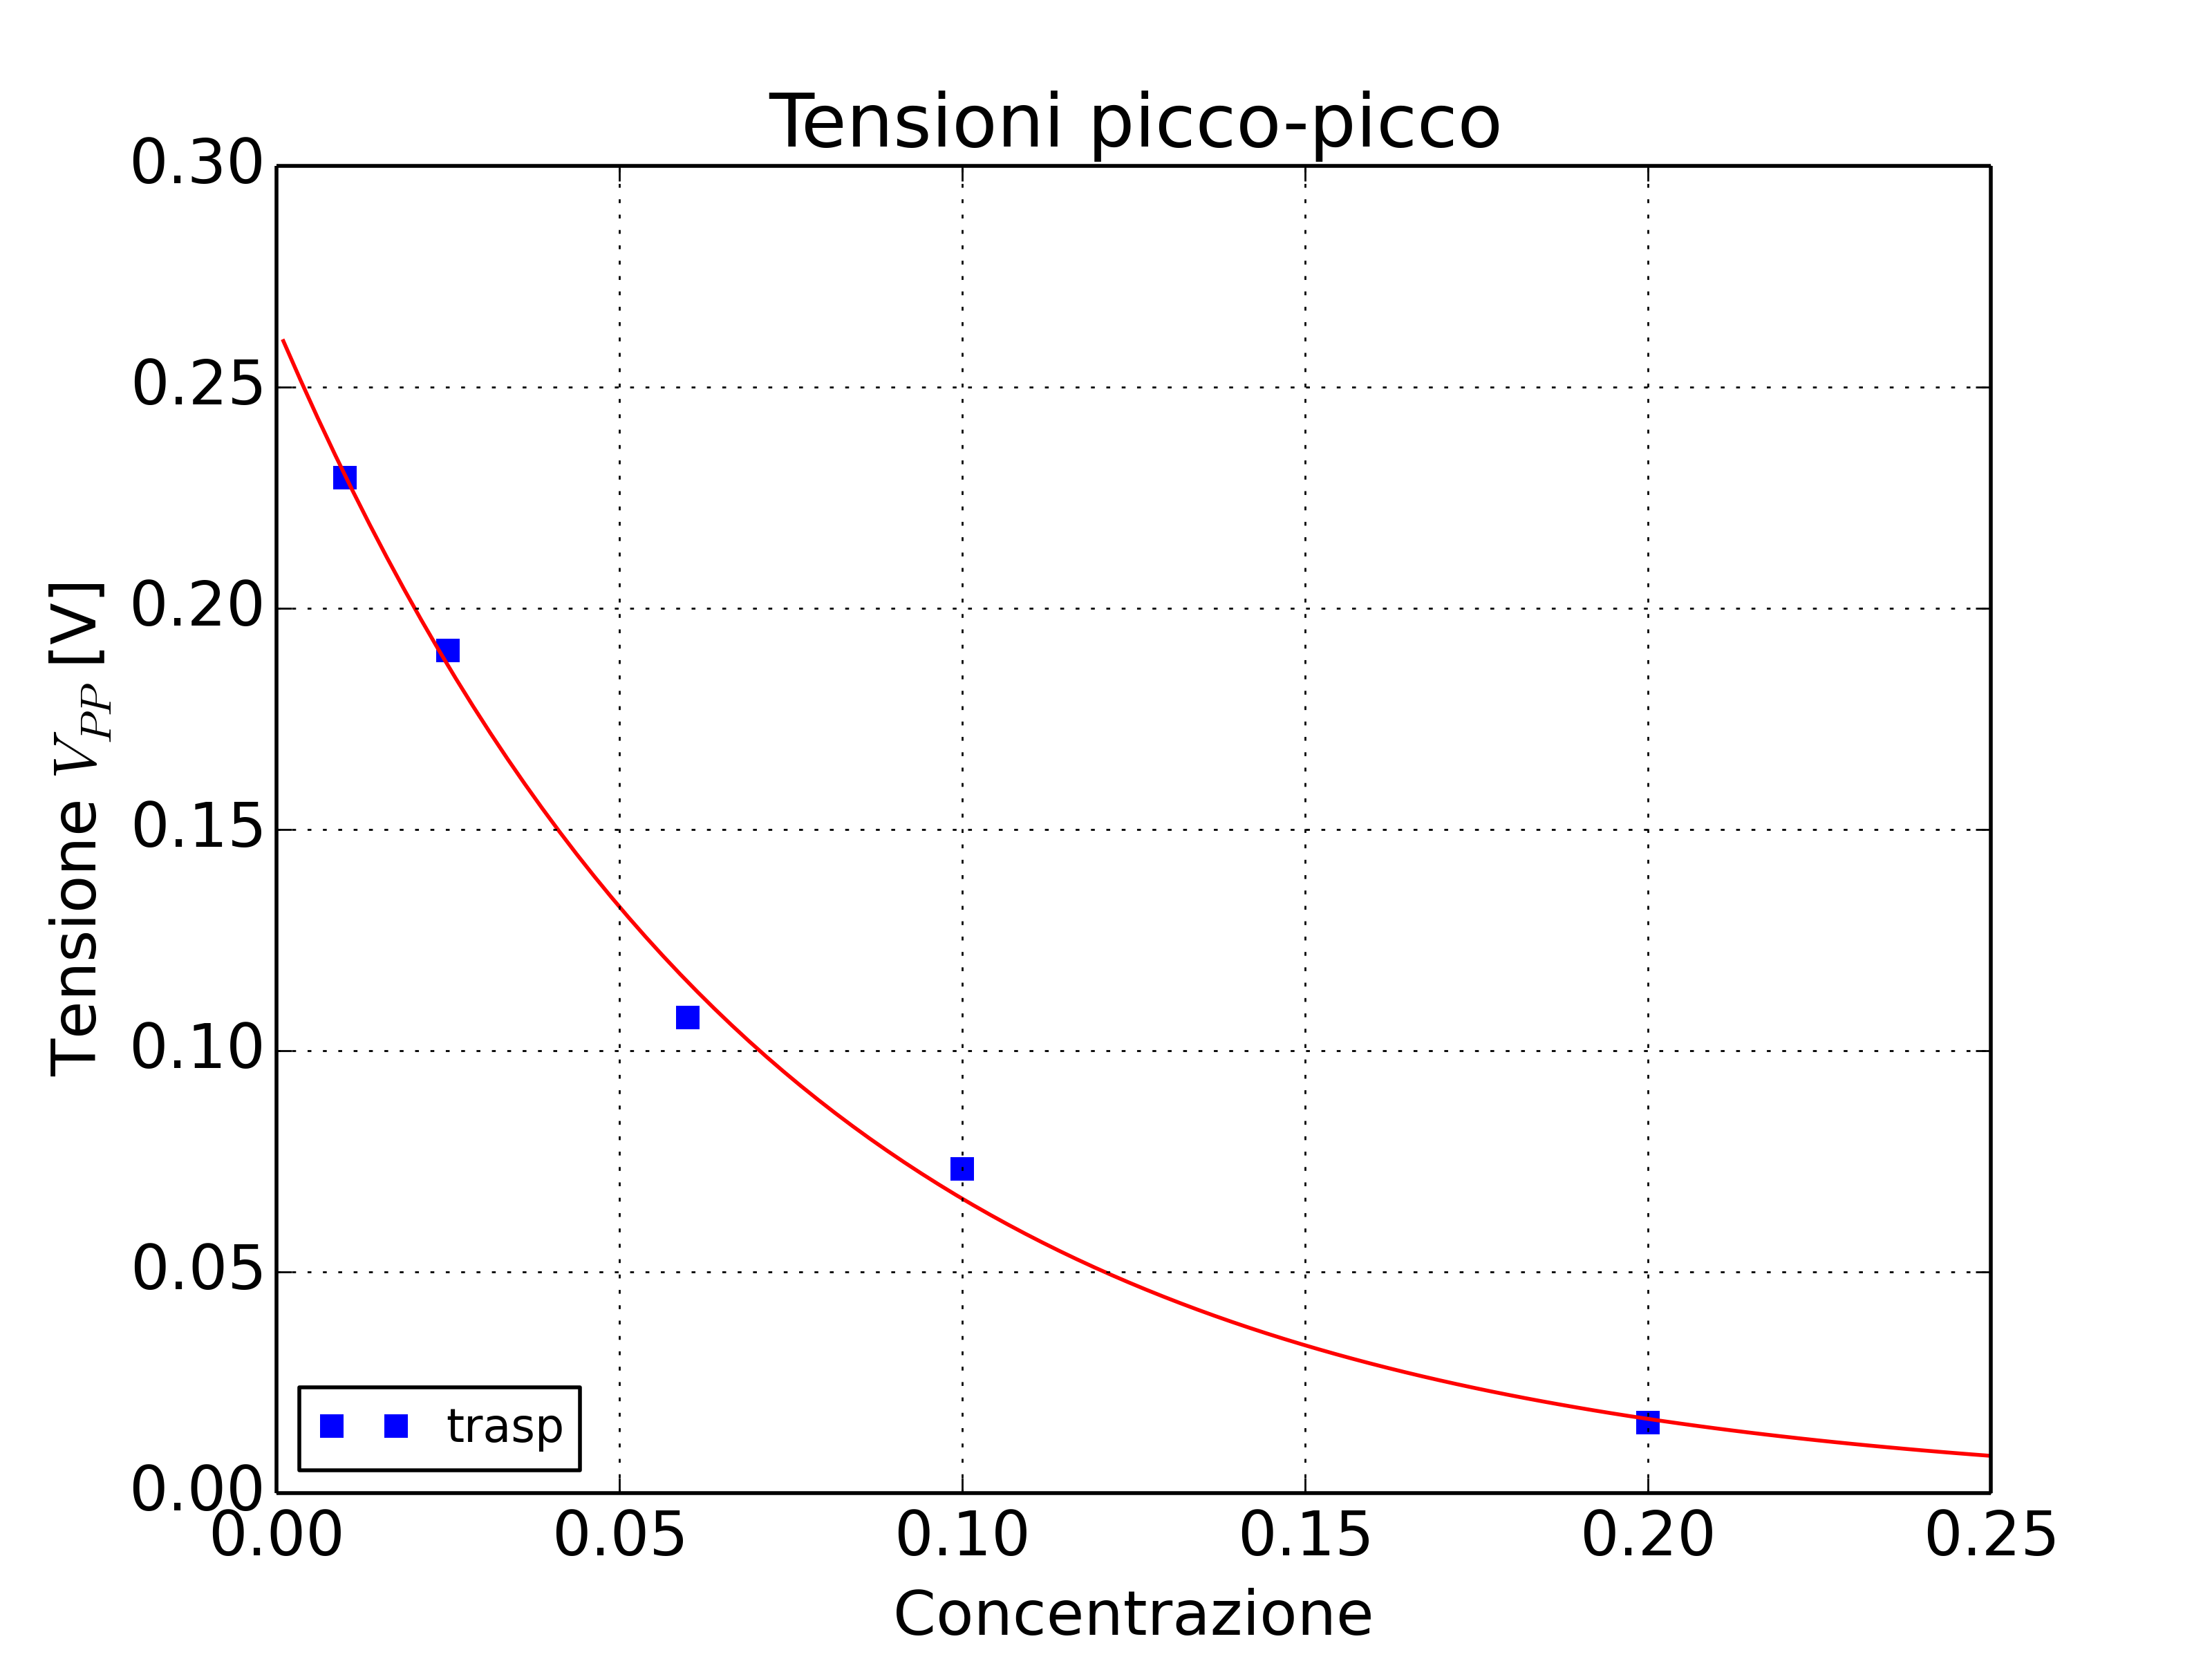
\includegraphics[width=0.7\linewidth]{./es13_tens_piccopicco_plot_mod}
\caption{Fit delle tensioni picco-picco in funzione delle concentrazioni (sicuramente scambiate).}
\label{fig:es13_tens_piccopicco_plot_mod}
\end{figure}


\subsection{Procedura di averaging}
L'idea alla base di questo metodo è molto semplice: sommando un elevato numero di acquisizoni dove vi è del rumore comparabile al livello del segnale oscillante, si ha che la parte del \textit{noise} tenderà ad annullarsi poichè questo è a media nulla e con fluttuazioni casuali al di sopra o al di sotto dello zero, mentre invece la modulazione si sommerà costruttivamente rendendo evidente il segnale (infine si divide per il numero di iterazioni per ottenere i livelli medii).\\
Per impiegare questa procedura usiamo il VI \textsc{diodolasr\_modulato}, che prevede un'ulteriore opzione che dovrebbe migliorare la qualità dell'averaging: vale a dire la possibilità di usare un secondo canale (nel nostro caso il CHB dell'ATTEN) come trigger per sincronizzare le acquisizioni. Il trigger può essere attivato o disattivato. Eseguendo varie misure è possibile scrivere alcune osservazioni generali:

\begin{itemize}
\item All'aumentare del numero di iterazioni la qualità del segnale ricostruito aumenta in maniera sensibile, anche se questo risulta particolarmente evidente per ampiezze di modulazione non troppo piccole  e per concentrazioni non superiori ad 1M.
%: come si vede dalle Figure () se queste ultime due condizioni non sono rispettate, la forma d'onda ricostruita è piuttosto scarsa;

\item Si nota un miglioramento all'attivarsi del trigger, tuttavia questo non è pronunciato ed effettivamente il suo effetto è visibile solo per un basso numero di iterazioni (inferiore a 50-100). 
\end{itemize}

E' interessante valutare quale potrebbe essere il minimo segnale rivelabile con tale metodologia: impieghiamo ovviamente la concentrazione 1.0M, con ampiezze 300mV e 50mV, e quella 1.2M, con due modulazioni di ampiezza 10mV e 1mV (il minimo fornito dal generatore ATTEN). I risultati di queste prove sono mostrati nelle Figure (\ref{fig:minimo_rivelabile}). Ad 1mV è ancora visibile un residuo di segnale che, tuttavia, ha una forma d'onda davvero distorta e assolutamente non periodica.


\begin{figure}
\centering
\subfloat[Subfigure 1 list of figures text][]{
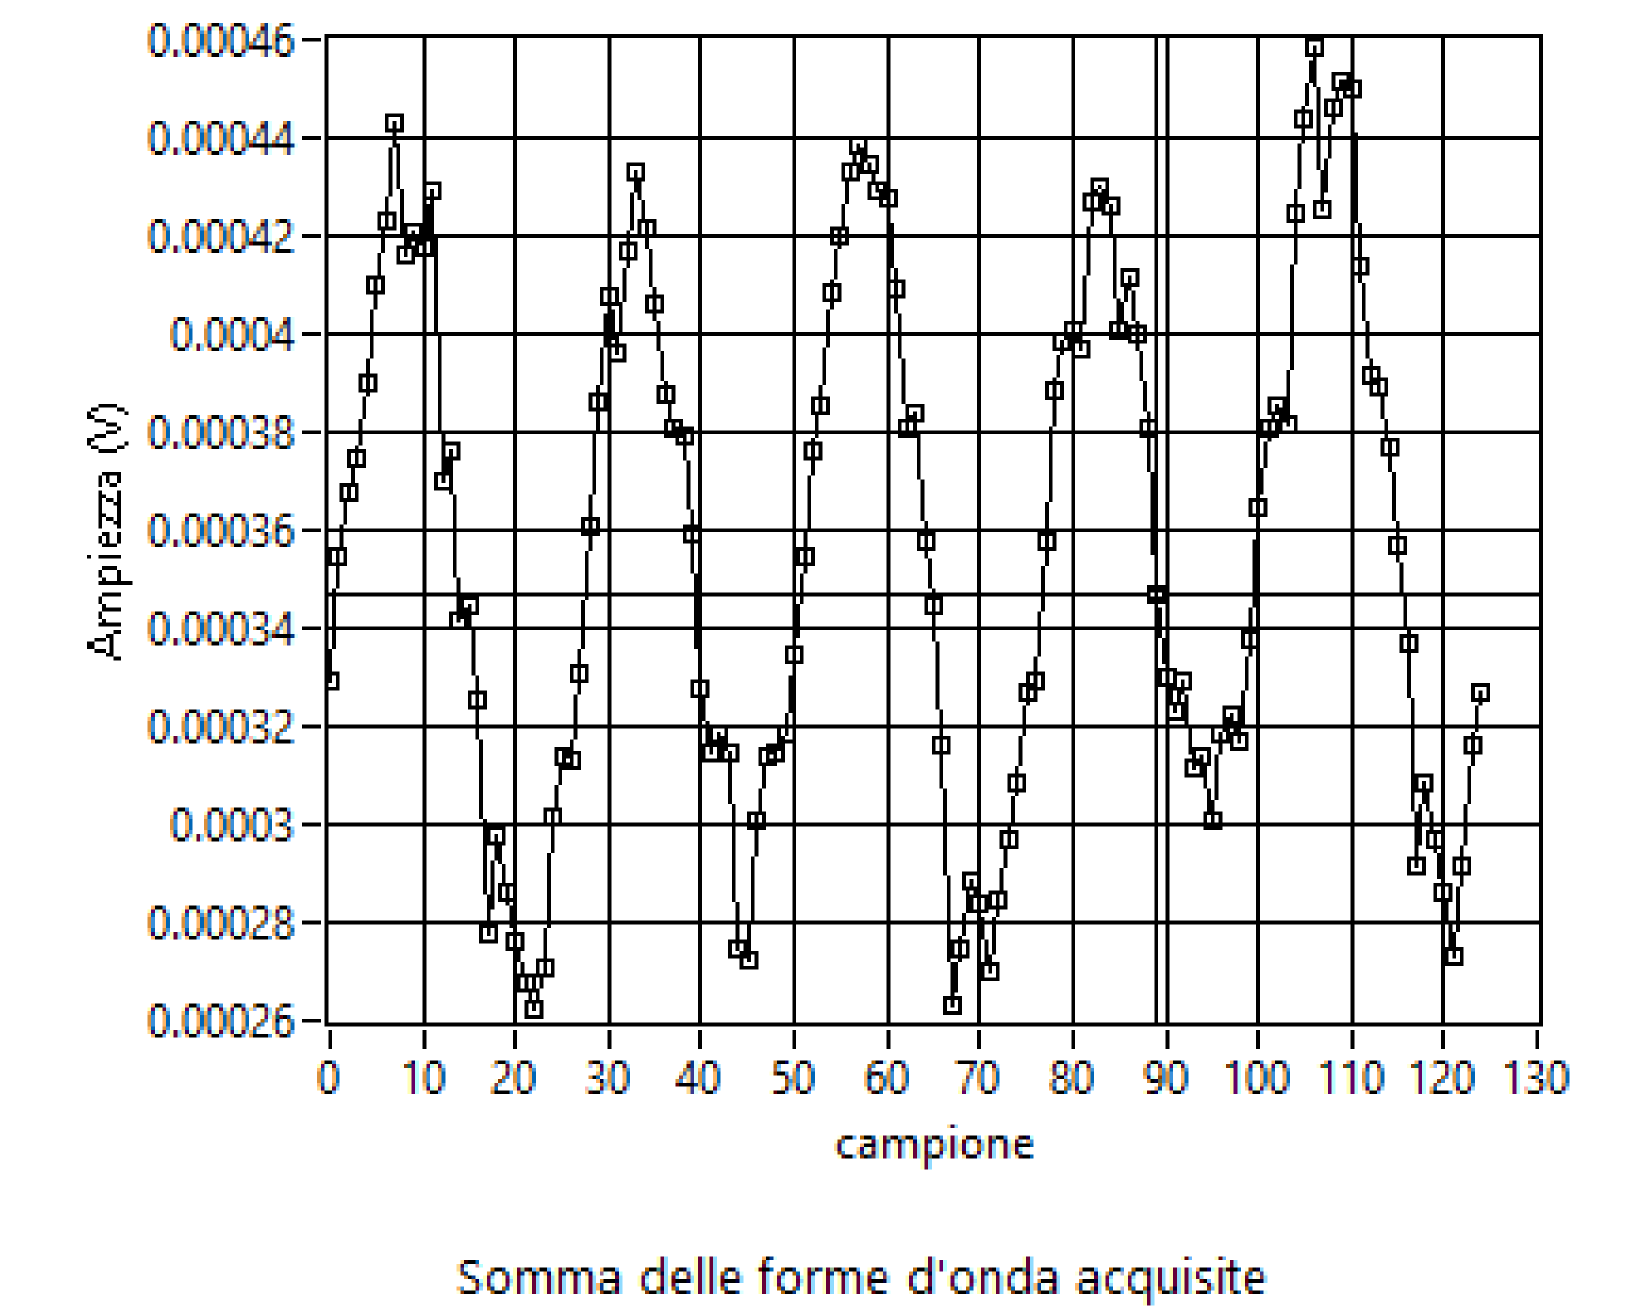
\includegraphics[width=0.5\linewidth]{./es14_1000iter_trig_cuv_1M_300mV}
\label{1000 iterazioni, 1M, 300mV}}
%\qquad
\subfloat[Subfigure 2 list of figures text][]{
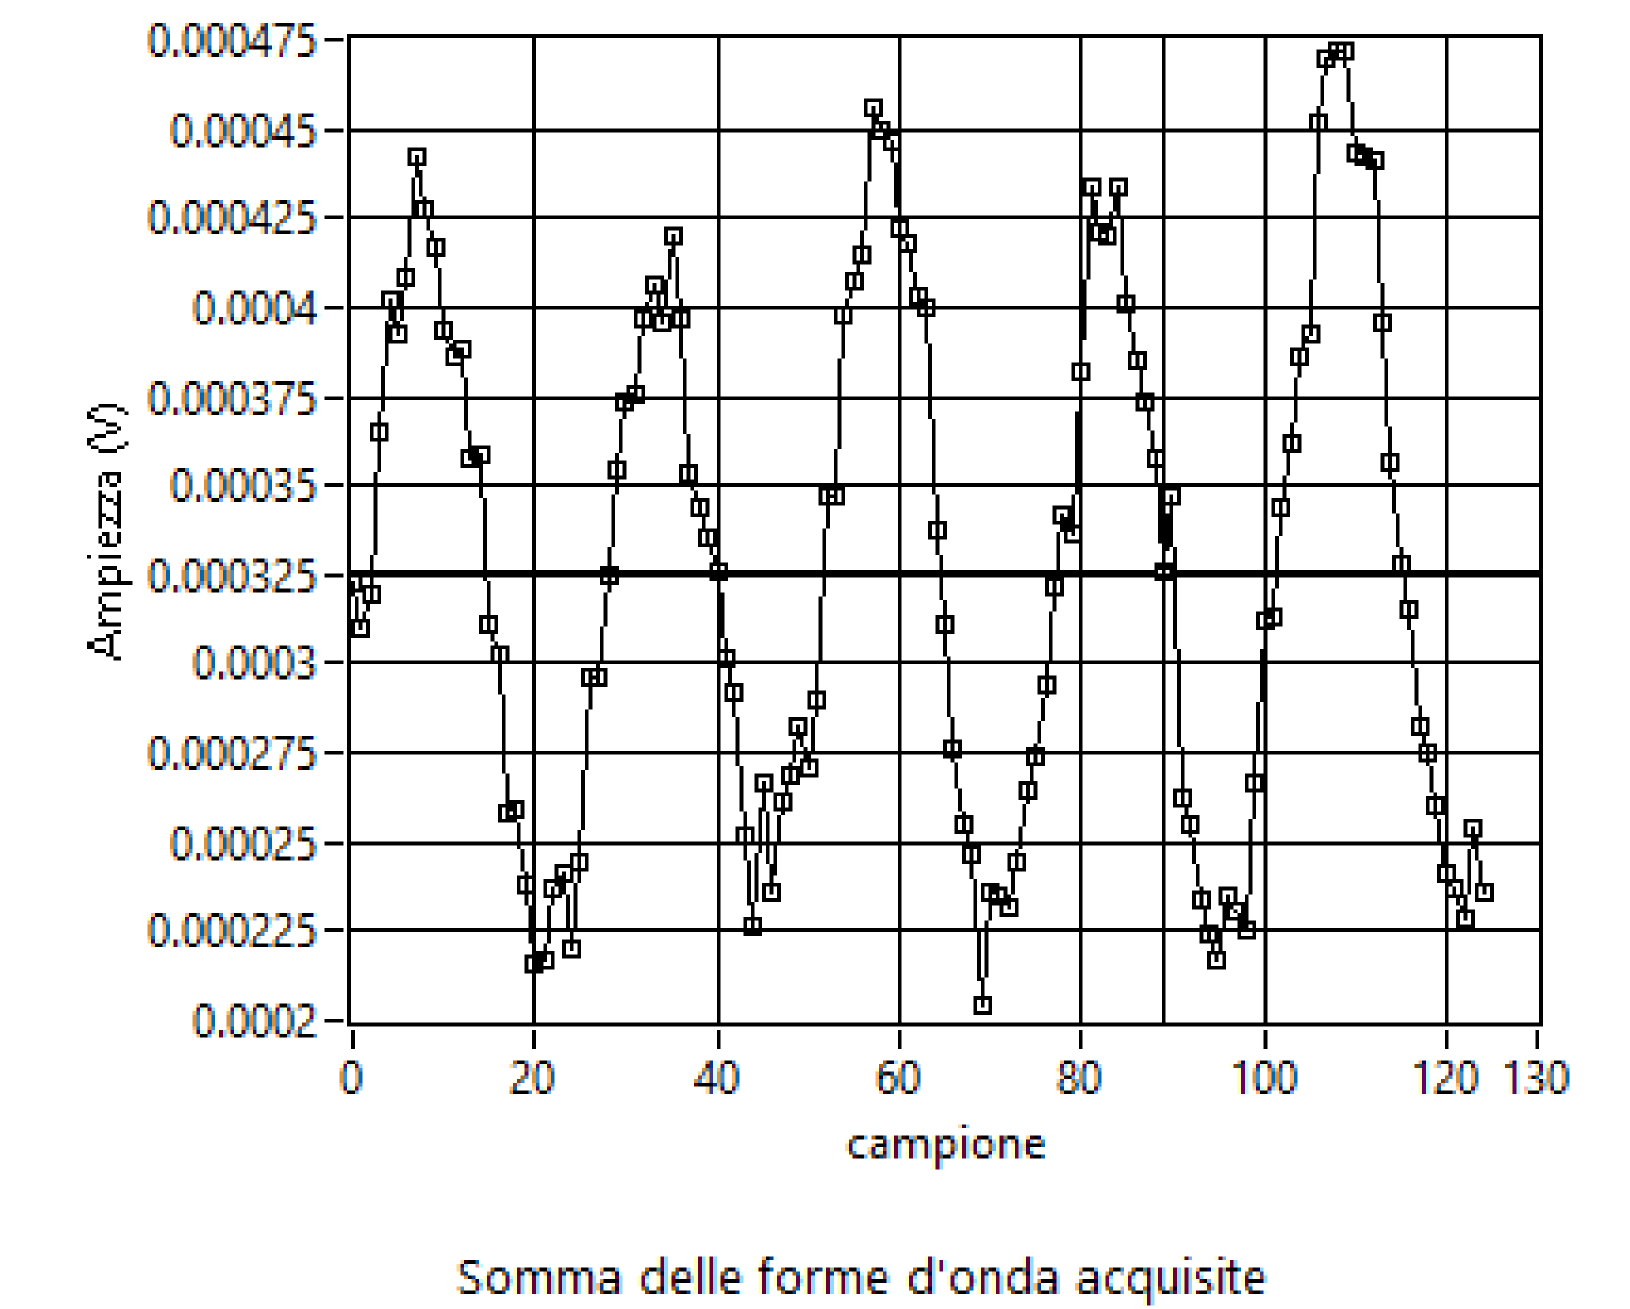
\includegraphics[width=0.5\linewidth]{./es14_200iter_trig_cuv_1M_50mV}
\label{200 iterazioni, 1M, 50mV}}
\qquad

\subfloat[Subfigure 1 list of figures text][]{
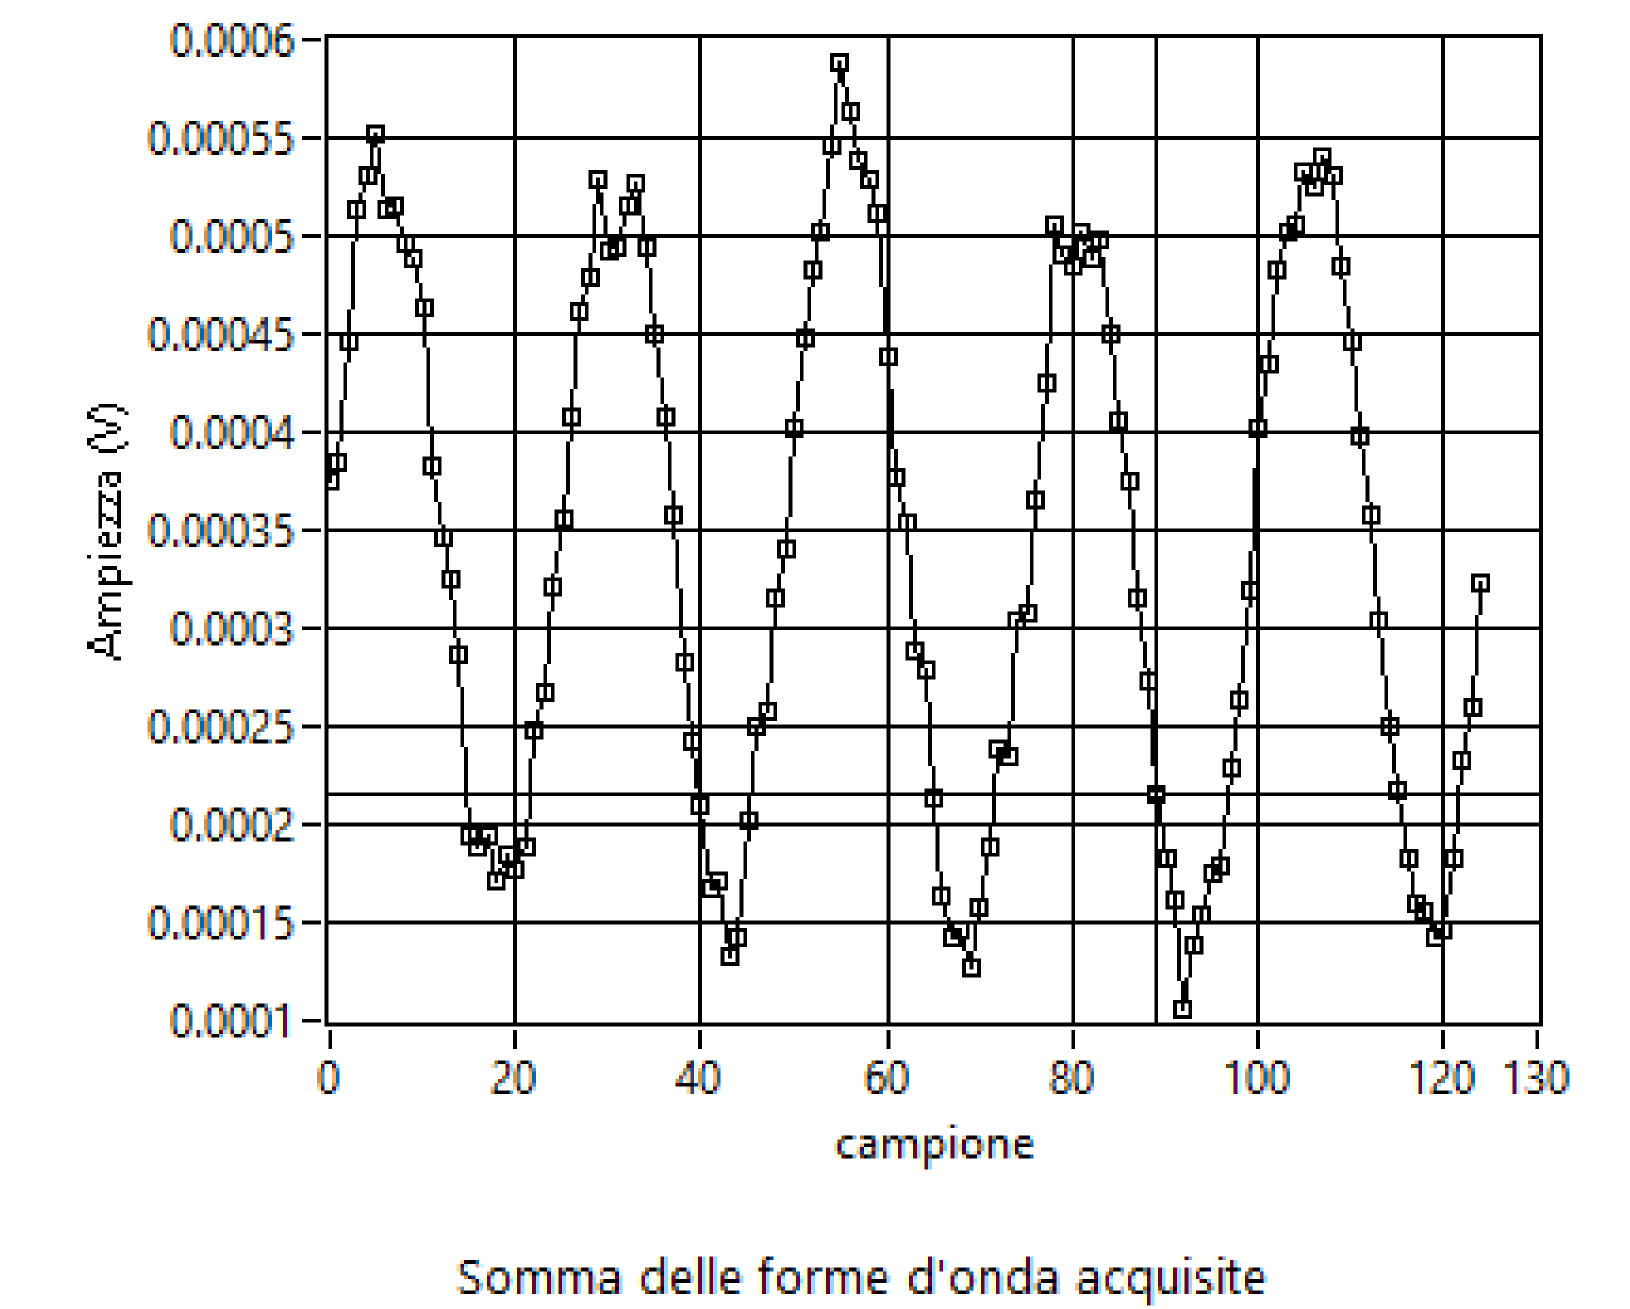
\includegraphics[width=0.5\linewidth]{./es14_200iter_trig_cuv_1_2M_10mV}
\label{200 iterazioni, 1.2M, 10mV}}
%\qquad
\subfloat[Subfigure 2 list of figures text][]{
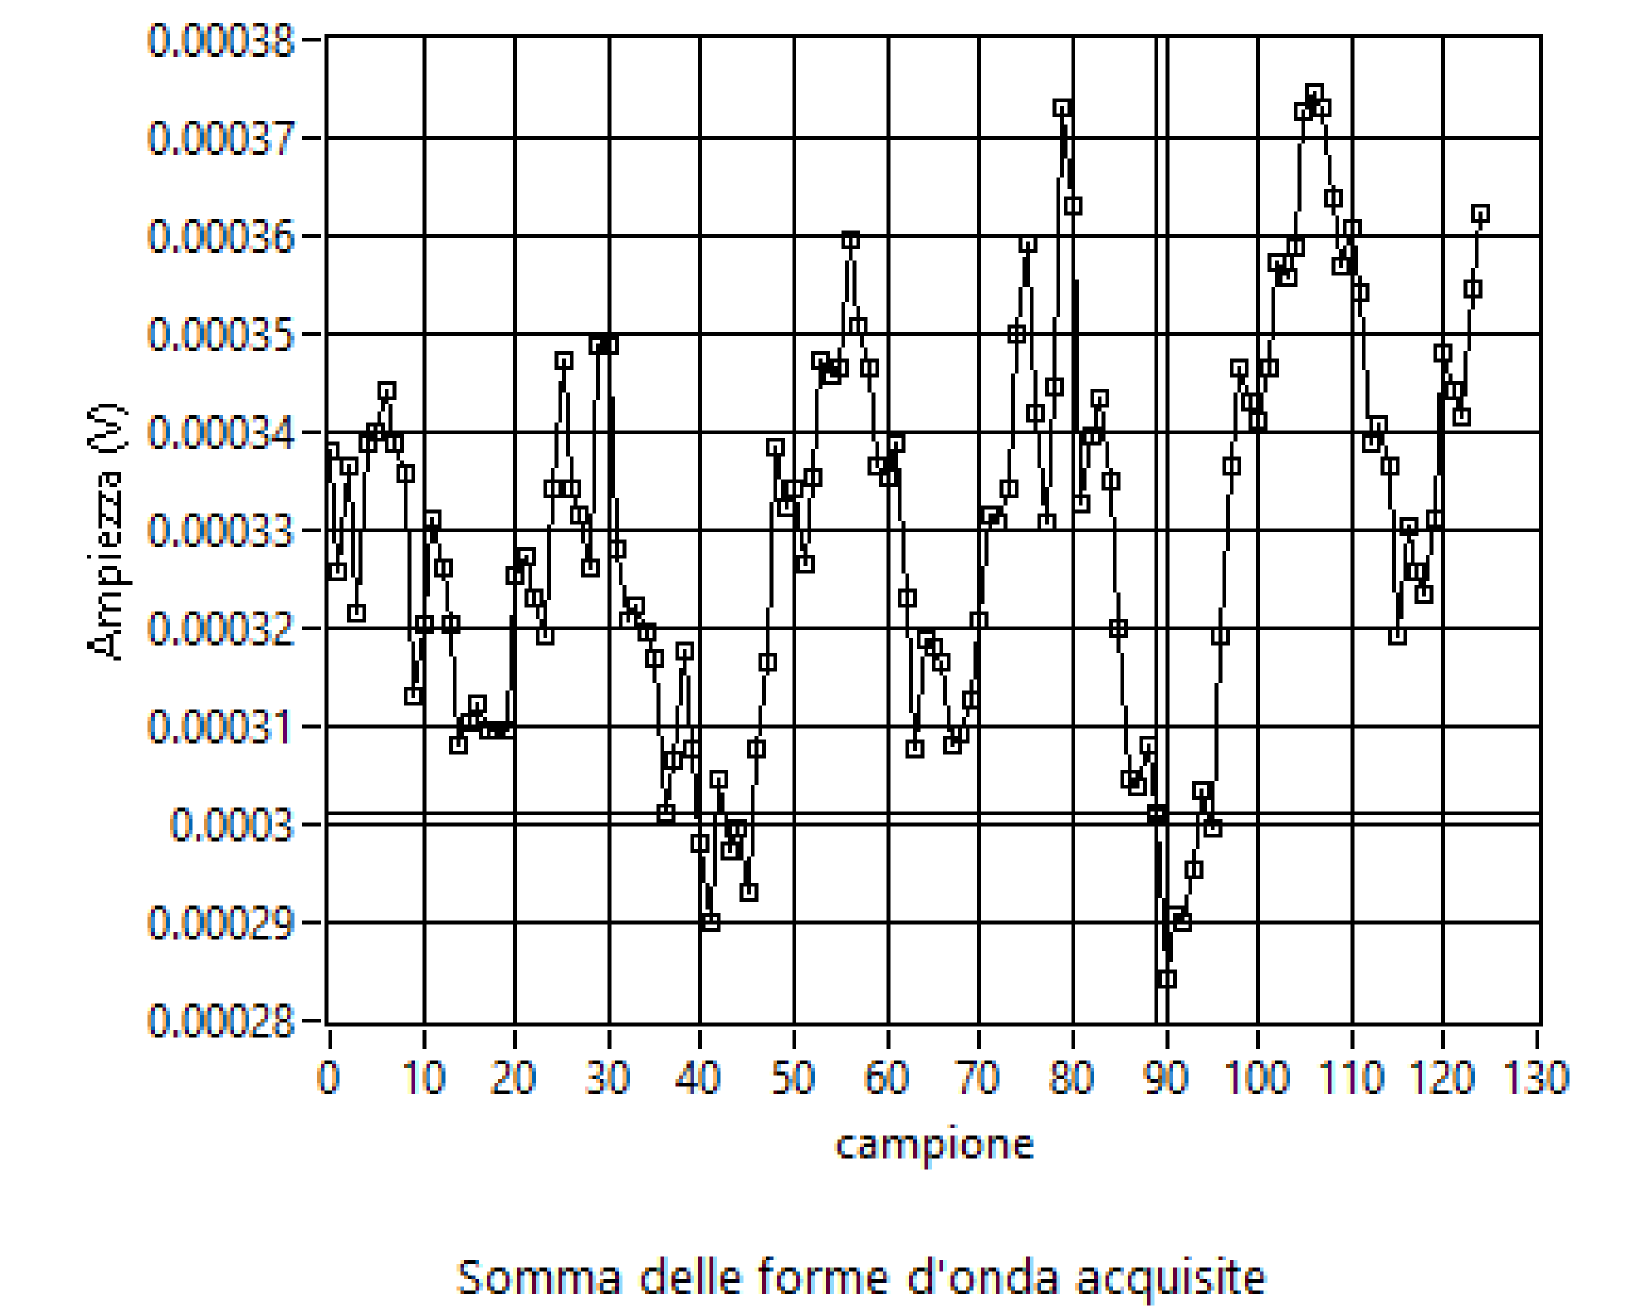
\includegraphics[width=0.5\linewidth]{./es14_1000iter_trig_cuv_1_2M_1mV}
\label{1000 iterazioni, 1.2M, 1mV}}

\caption{Minimo segnale rivelabile.}
\label{fig:minimo_rivelabile}
\end{figure}


\section{Rivelazione di piccoli segnali - II}
Il secondo metodo che useremo per rivelare i piccoli segnali è decisamente più raffinato e vicino alla procedura standard di lock-in: si utilizza l'integrato \textsc{ad633} della \textbf{Analog Devices} che, come scritto ben in evidenza sul datasheet, è un \textit{low cost analog multiplier}. Questo componente permette di eseguire il prodotto di due segnali posti agli ingressi e di restituire il risultato in uscita. In realtà la questione è ancora più interessante, dal momento che i due ingressi sono di tipo differenziale e vi è la possibilità di sommare un ulteriore segnale al prodotto dei primi due. In base a quanto mostrato in Figura (\ref{fig:schema_ad633}), che è quella corrispondente al package \textit{Lead PDIP} in nostro possesso, l'output dell'integrato è dato dalla formula:\\

\begin{equation}
\textbf{W} = \frac{(\textbf{X}_1 - \textbf{X}_2)(\textbf{Y}_1 - \textbf{Y}_2)}{10\mathrm{V}} + \textbf{Z}
\end{equation}

\begin{figure}
\centering
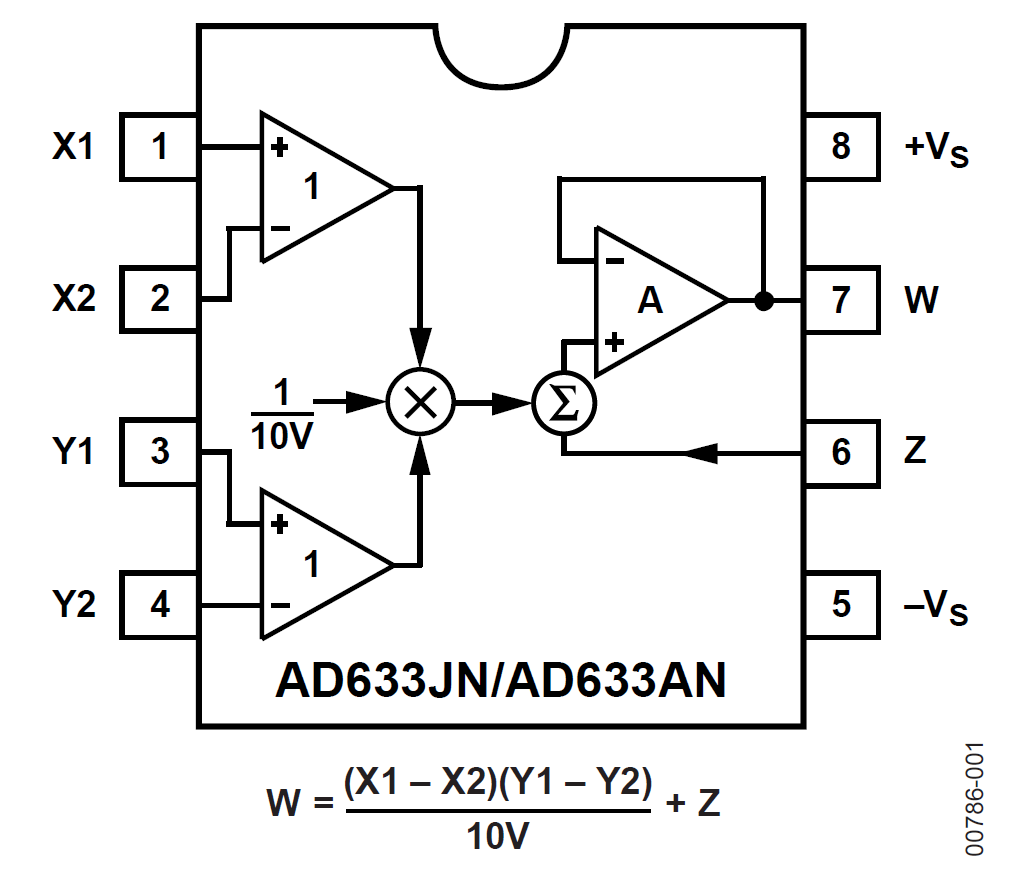
\includegraphics[width=0.4\linewidth]{./schema_ad633}
\caption{Schema dell'AD633, packaging Lead PDIP.}
\label{fig:schema_ad633}
\end{figure}


Riportiamo di seguito alcune specifiche di funzionamento:

\begin{table}
\centering
\begin{tabular}{c|c}
\hline \textbf{Parameter} & \textbf{Values} \\ 
\hline Supply Voltage & $\pm 8 - \pm 18$ V (rated $\pm 15$V) \\ 
 Input Offset Voltage & 5-30 mV \\ 
 Output Offset Voltage & 5-50 mV \\  
 Small Signal Banwidth & 1MHz @ V = 0.1V rms \\
\hline
\end{tabular} 
\end{table}
~\\

Proviamo qualche configurazione di test dell'integrato, in modo da prendere confidenza con le sue proprietà.\\
Come primo tentativo vogliamo produrre un'uscita di frequenza doppia in W. Vi sono sicuramente diversi modi per farlo, tra i più facili da realizzare si hanno:

\begin{itemize}
\item Si collegano $X_2$, $Y_2$, $Z$ a GND e si manda ad entrambi gli ingressi $X_1$ e $Y_1$ lo stesso segnale sinusoidale di frequenza $\omega$. Per la funzione di trasferimento riportata sopra, è evidente che l'uscita W sarà il $\sin^2 \omega t$ riscalato di una certa costante moltiplicativa, che per le note formule di bisezione si può scrivere come $(1- \cos 2\omega t)2$, che ovviamente è un segnale a frequenza doppia. L'inconveniente è che vi è un offset continuo che può risultare scomodo.

\item Una seconda possibilità è quella di (lasciando a GND $X_2$, $Y_2$, $Z$) mandare a $X_1$ e $Y_1$ lo stesso segnale ma sfasato di $\pi/2$ e moltiplicare, in sostanza, un $\sin \omega t$ e un $ \cos \omega t$, di modo che il prodotto abbia frequenza doppia ma niente offset. Il principale svantaggio di questo metodo è che è difficile produrre separatamente due segnali perfettamente sfasati di 90° e della stessa frequenza, per cui anche minime deviazioni iniziali nel lungo periodo danno luogo a fenomeni di battimenti e creazione di fondi continui.
\end{itemize} 


In Figura (\ref{fig:es19_sinquadro}) si è riportato il risultato in uscita avendo collegato ai due ingressi lo stesso segnale, come spiegato al punto (i): si nota la presenza di un offset al segnale a frequenza doppia.\\

\begin{figure}
\centering
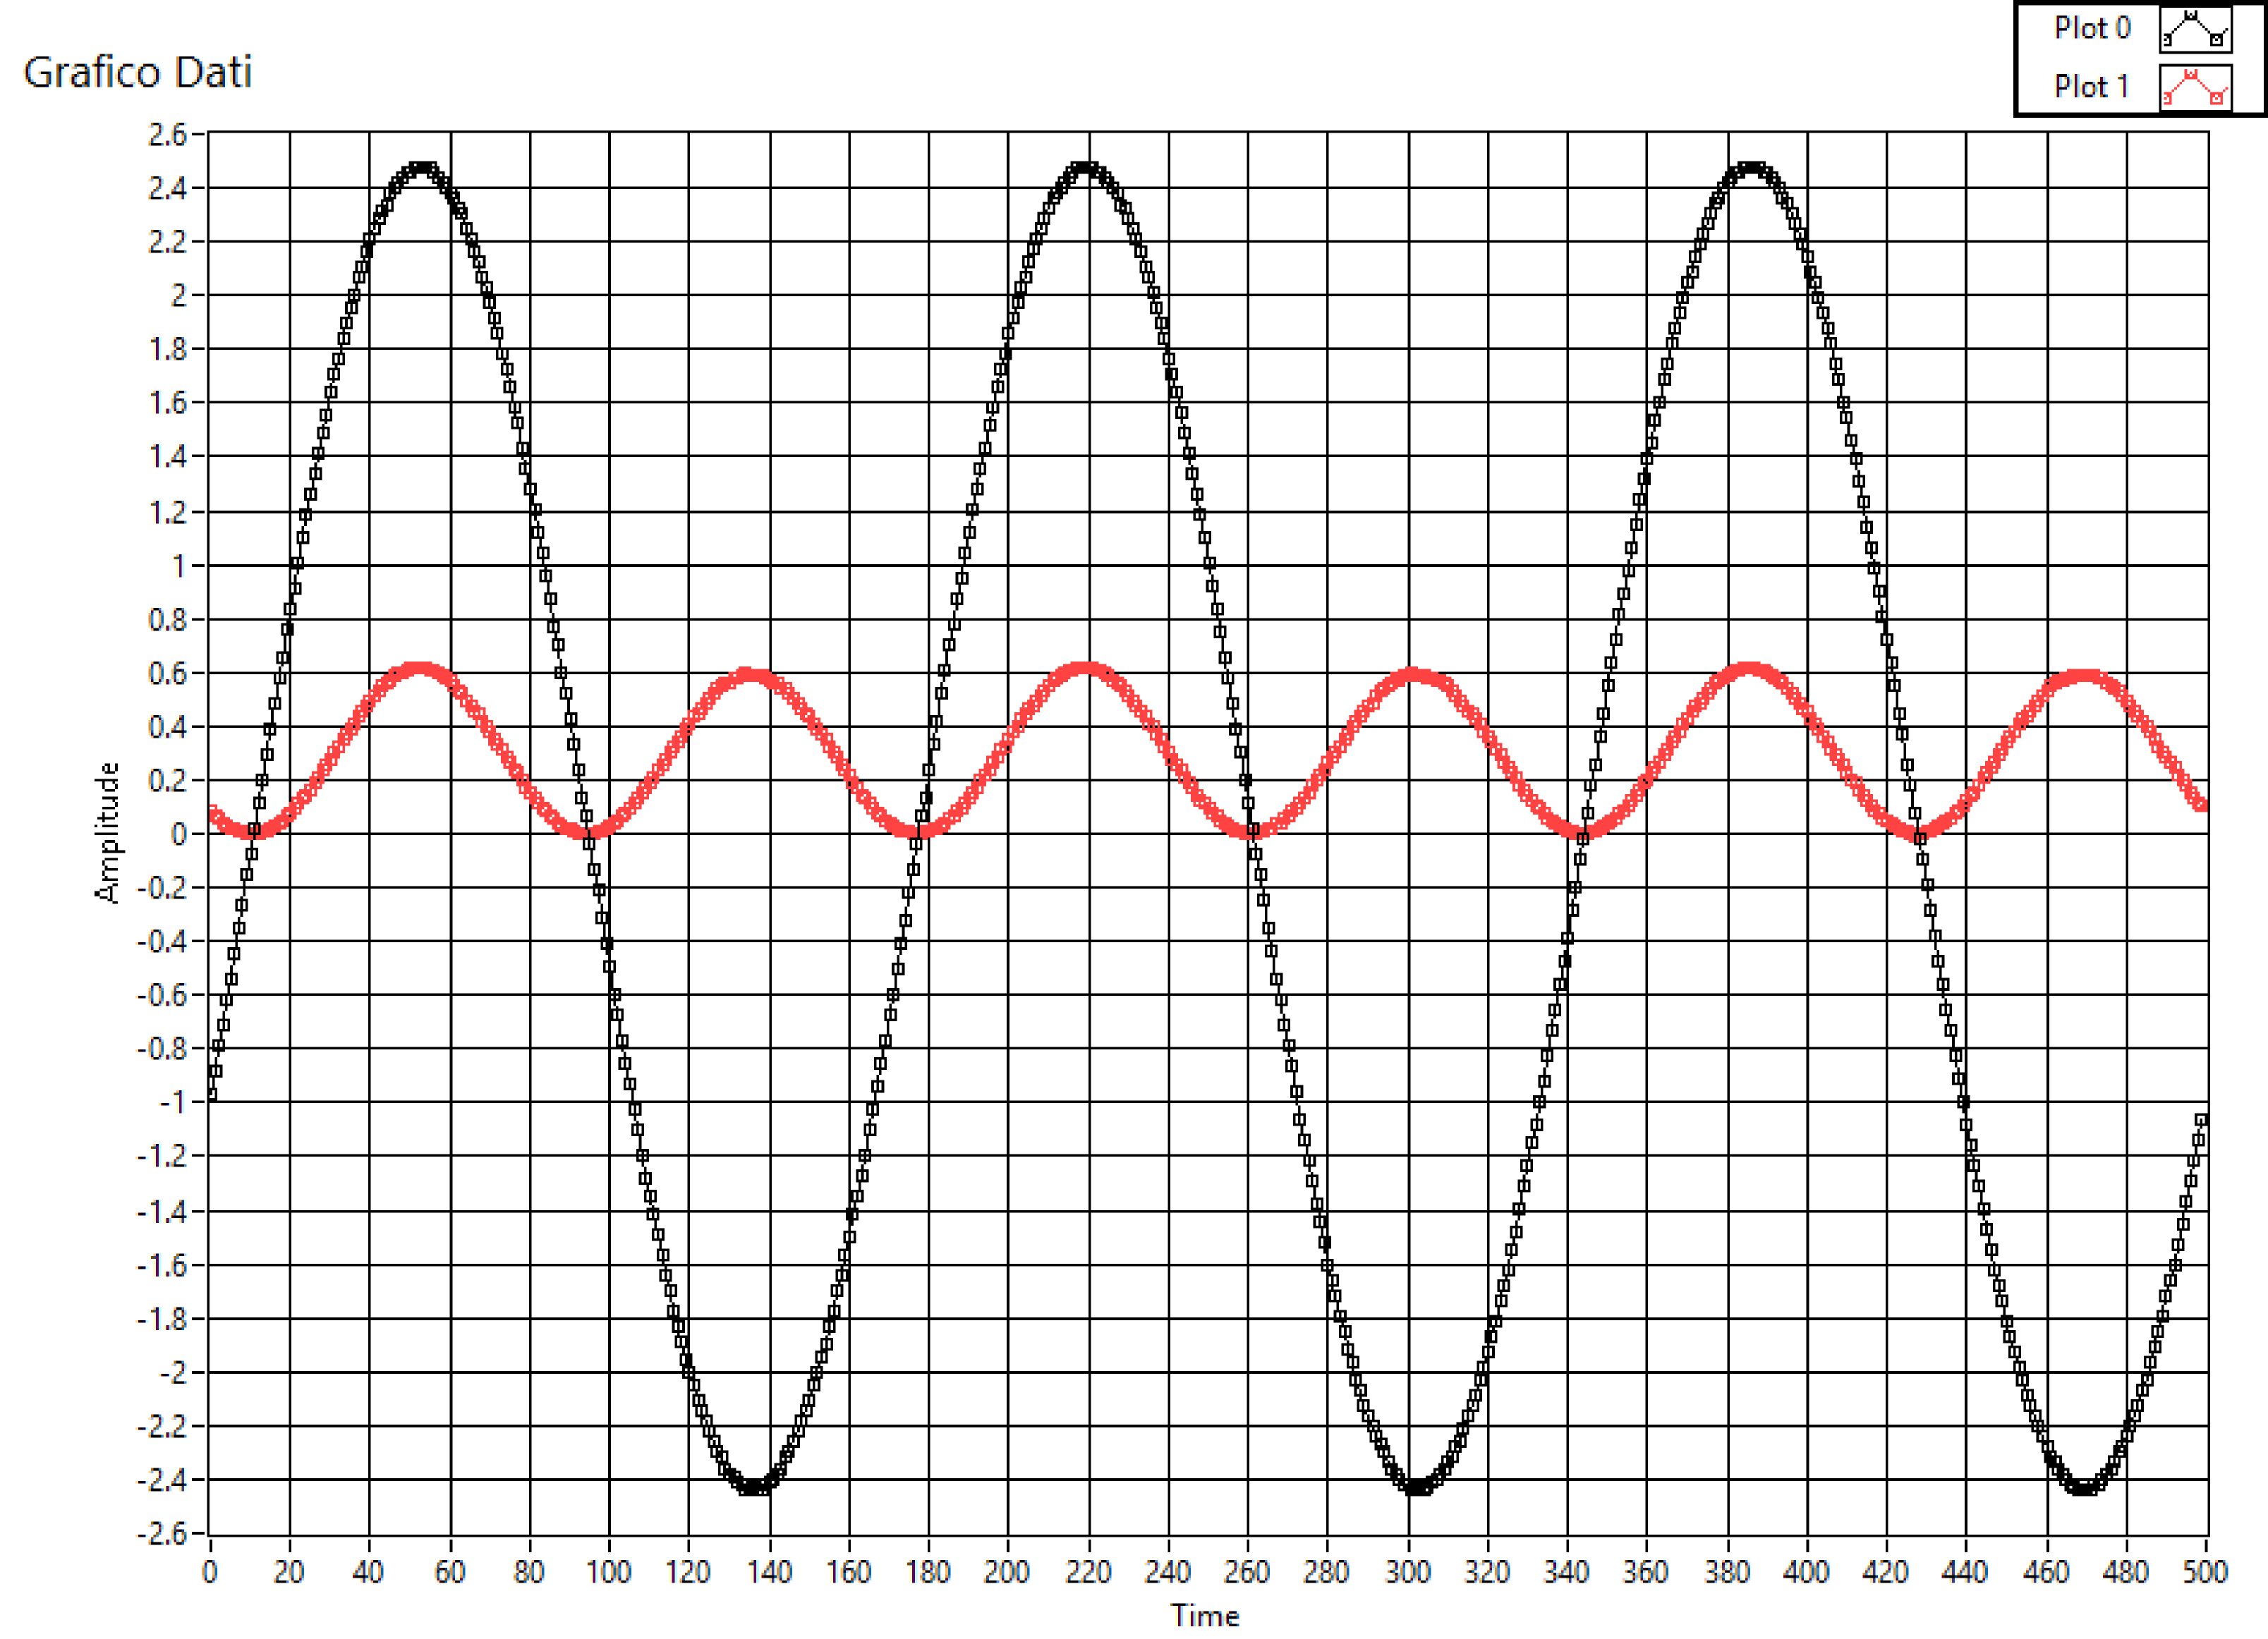
\includegraphics[width=0.8\linewidth]{./es19_sinquadro}
\caption{Generazione di un segnale a freqienza doppia con offset: in nero la tensione di ingresso con V=2.5V, l'uscita è data dalla linea rossa. Da notare che l'ampiezza finale è come aspettato $(2.5^2)/10 = 0.625 V$ che bisogna dividere per un ulteriore fattore 2 come risulta dalla formula di bisezione già menzionata.}
\label{fig:es19_sinquadro}
\end{figure}

Un modo furbo per eliminare l'offset e tuttavia continuare ad utilizzare lo stesso segnale di ingresso per $X_1$ e $Y_1$ è quello di mettere in uscita un filtro passa-alto che taglia la parte a basse frequenze (al limite frequenza nulla), e composto da un condensatore e una resistenza come in Figura (\ref{fig:es_20_togliere_offset}).\\

\begin{figure}
\centering
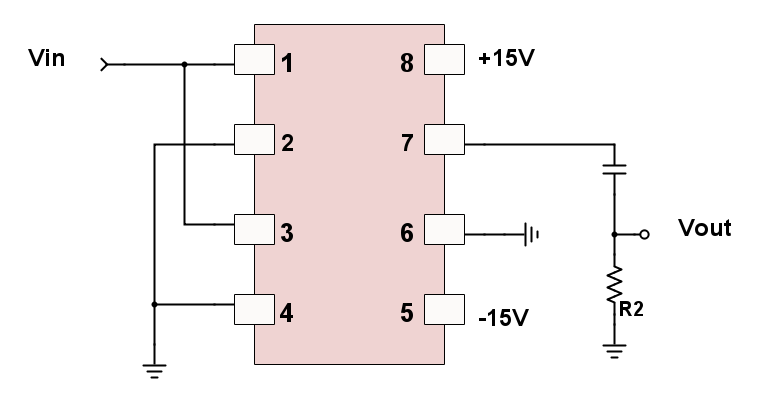
\includegraphics[width=0.8\linewidth]{./es_20_togliere_offset}
\caption{Uso di un filtor passa-alto per eliminare l'offset continuo in output}
\label{fig:es_20_togliere_offset}
\end{figure}


Allo stesso tempo sperimentiamo anche per la prima volta l'uso dell'ingresso Z per \textit{rinforzare} il segnale di output. Tuttavia, il nostro scopo è quello di ottenere una sinusiode ben definita in frequenza, per cui la tensione da sommare non può essere a caso, ma dovrà per forza essere la stessa in uscita. Si verifica a questo punto, però, un comportamento curioso dato che il segnale di rinforzo dipende da quello in uscita che dipende da quello di rinforzo che dipende da quello in uscita ecc... Si tratta chiaramente di una progressione geometrica che può convergere (e a noi ovviamente interessa che converga) solo per una ragione minore di 1: questo concretamente significa che il segnale di rinforzo deve necessariamente essere una frazione minore di 1 di quello di uscita e ciò si può ottenere con un partitore di tensione come in Figura (\ref{fig:es21}). \\



\begin{figure}
\centering
\subfloat[Subfigure 1 list of figures text][Partitore di tensione per rinforzare il segnale di uscita.]{
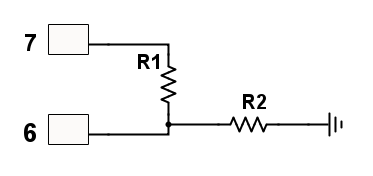
\includegraphics[width=0.5\linewidth]{./es21_partitore}
\label{fig:es21_partitore}}
%\qquad
\subfloat[Subfigure 2 list of figures text][Circuito complessivo con segnali sfasati di 90° in ingresso]{
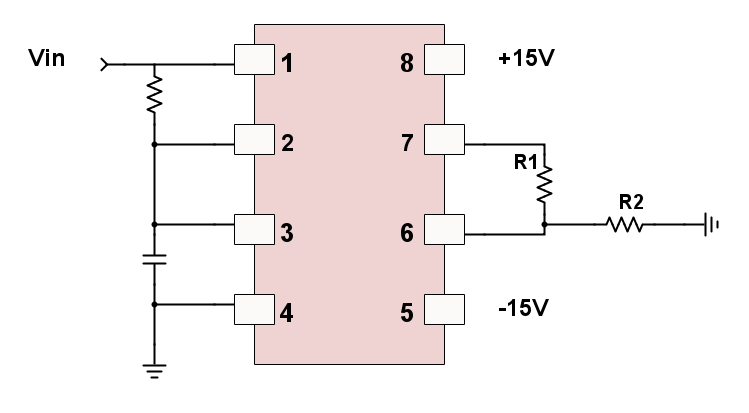
\includegraphics[width=0.5\linewidth]{./es21_rinforzo_completo}
\label{fig:es21_rinforzo_completo}}
%\qquad

\caption{Uso della porta Z per rinforzare il segnale; no offset in uscita.}
\label{fig:es21}
\end{figure}

Sia $q$ la frazione di tensione di output $V_O$ data dal partitore in Z, allora il segnale di uscita complessivo sarà:\\

\begin{equation}
V_{TOT} = V_O (1 + q + q^2 + q^3 + ...) = V_O \frac{1}{1-q}
\end{equation}


Il risultato per $q \simeq \left(3/4 , 10/11 \right) $ è molto gradevole ed è riportato in Figura (\ref{fig:es20_sub}).\\

\begin{figure}
\centering
\subfloat[Subfigure 1 list of figures text][Partitore 1-3 k$\Omega$]{
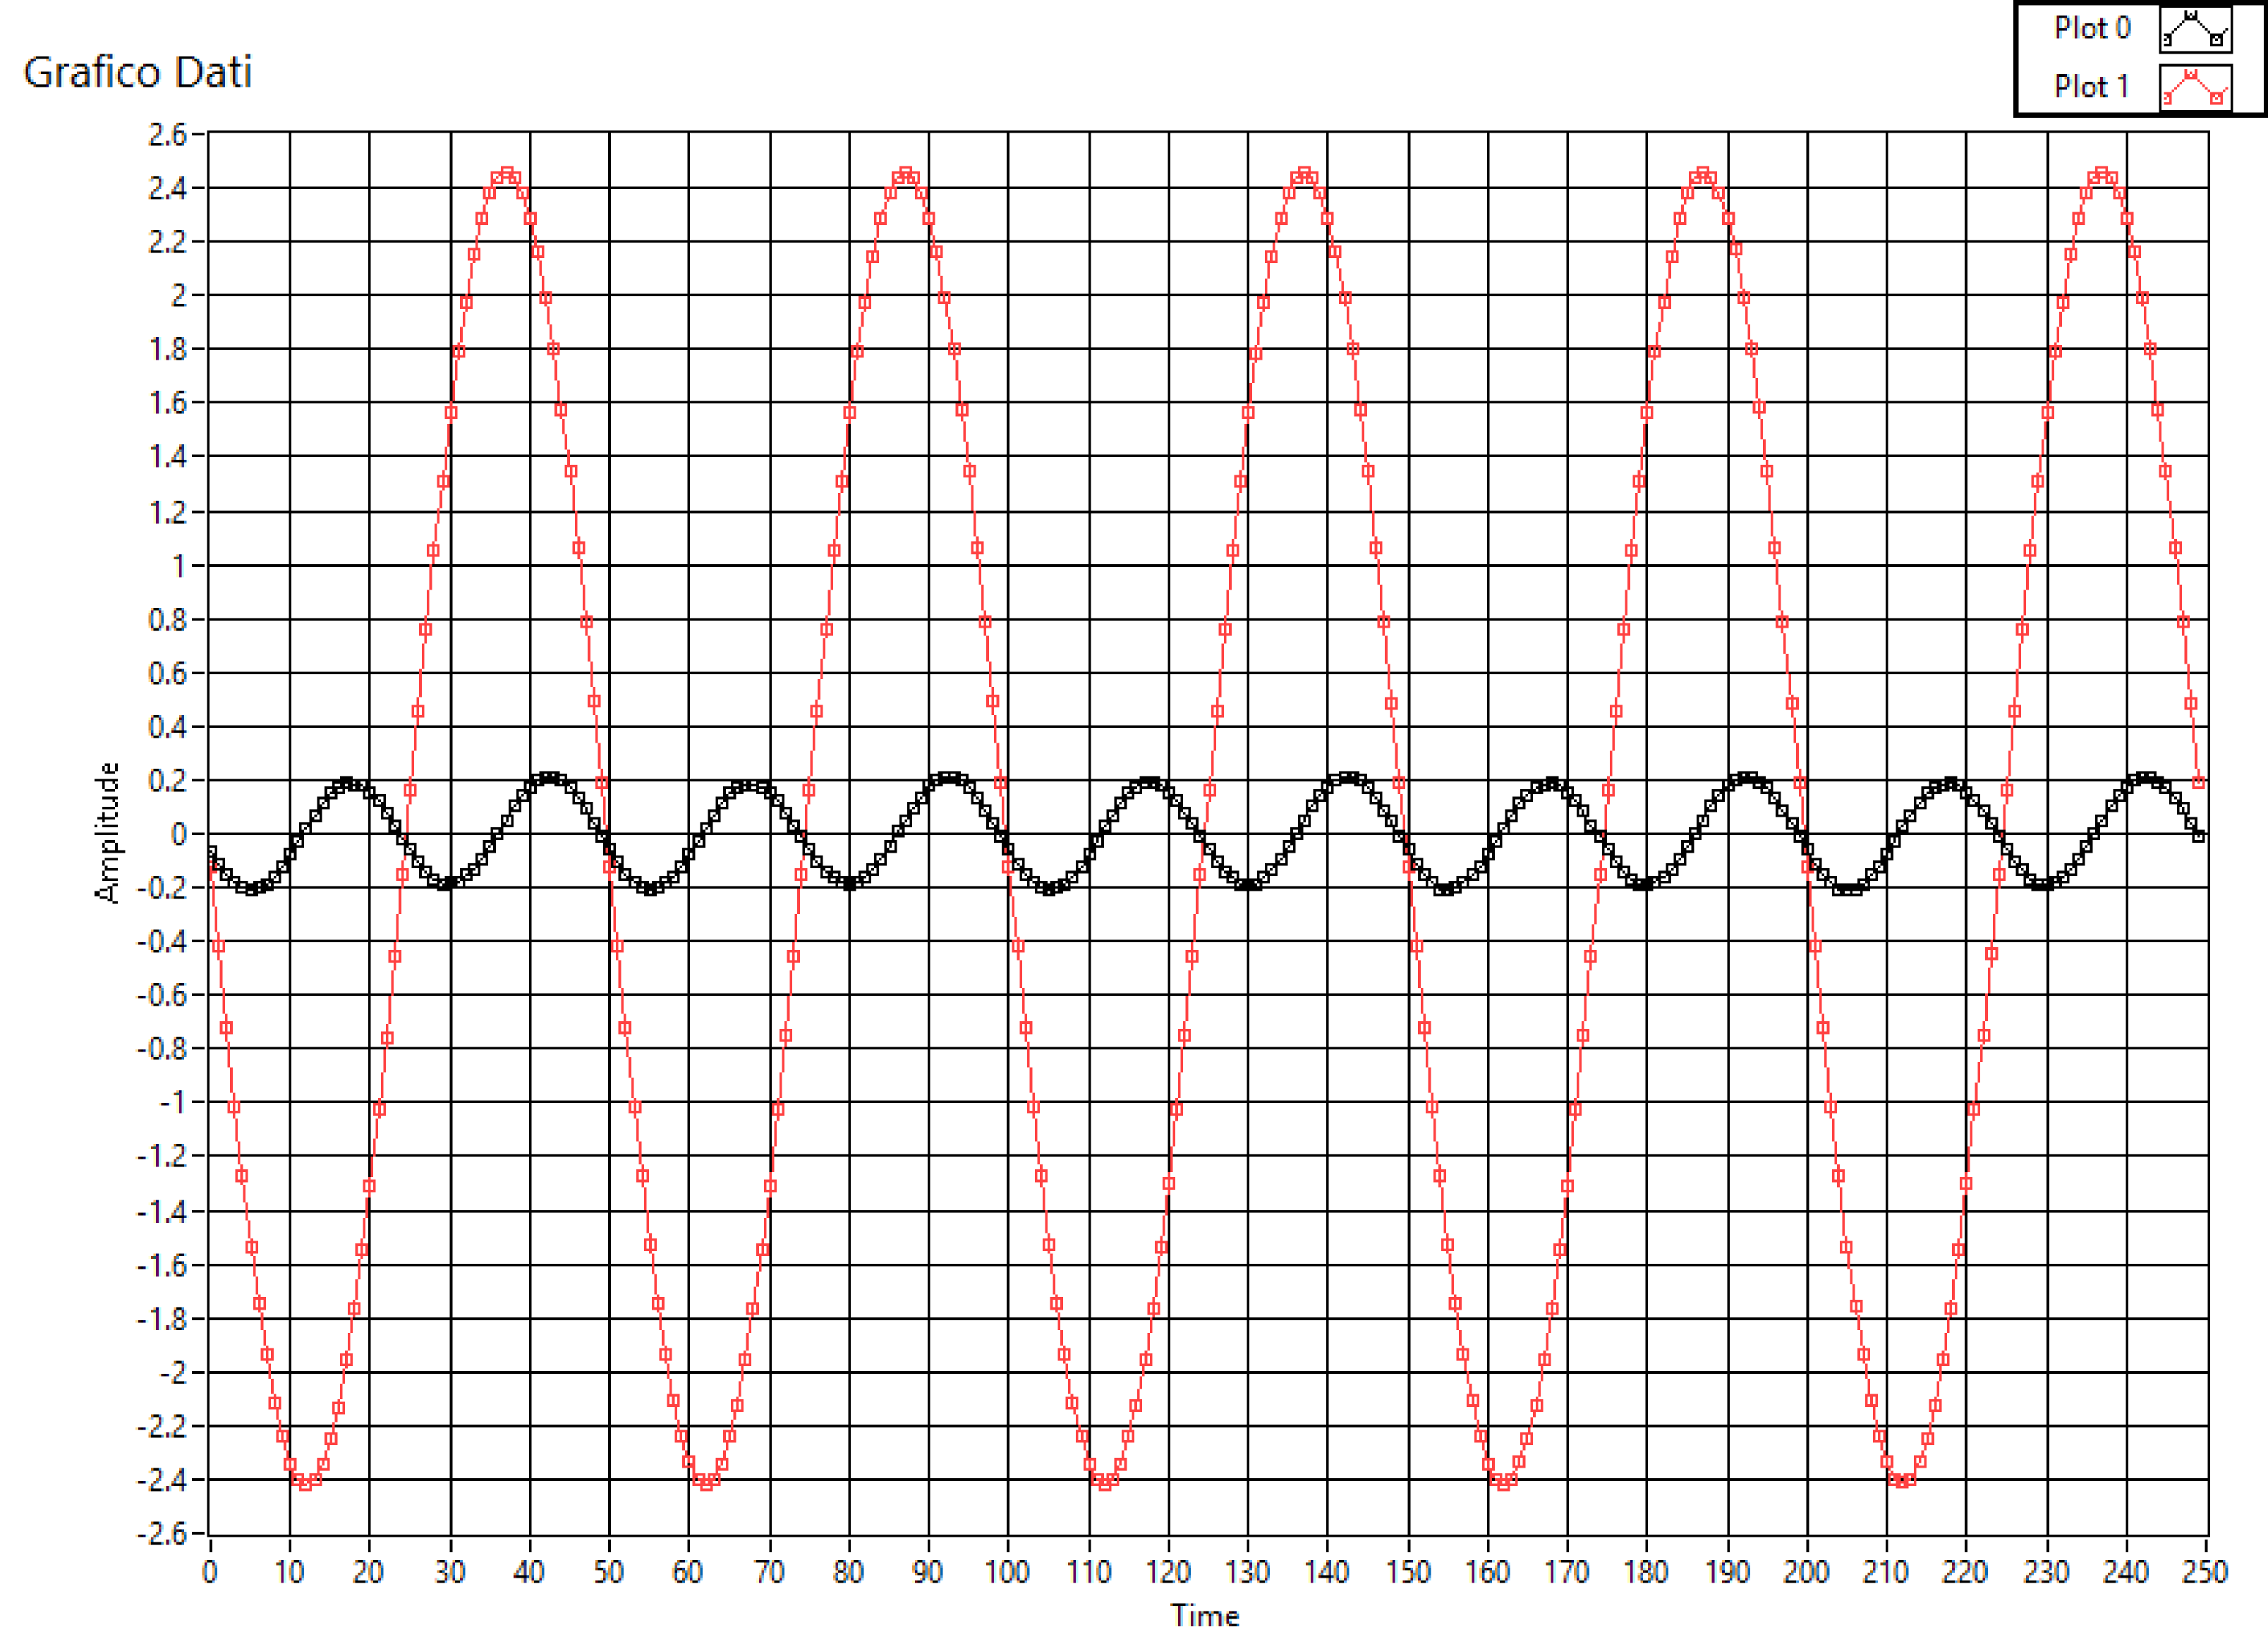
\includegraphics[width=0.5\linewidth]{./es20_part_1_3}
\label{fig:es20_fig}}
%\qquad
\subfloat[Subfigure 2 list of figures text][Partitore 1-10 k$\Omega$]{
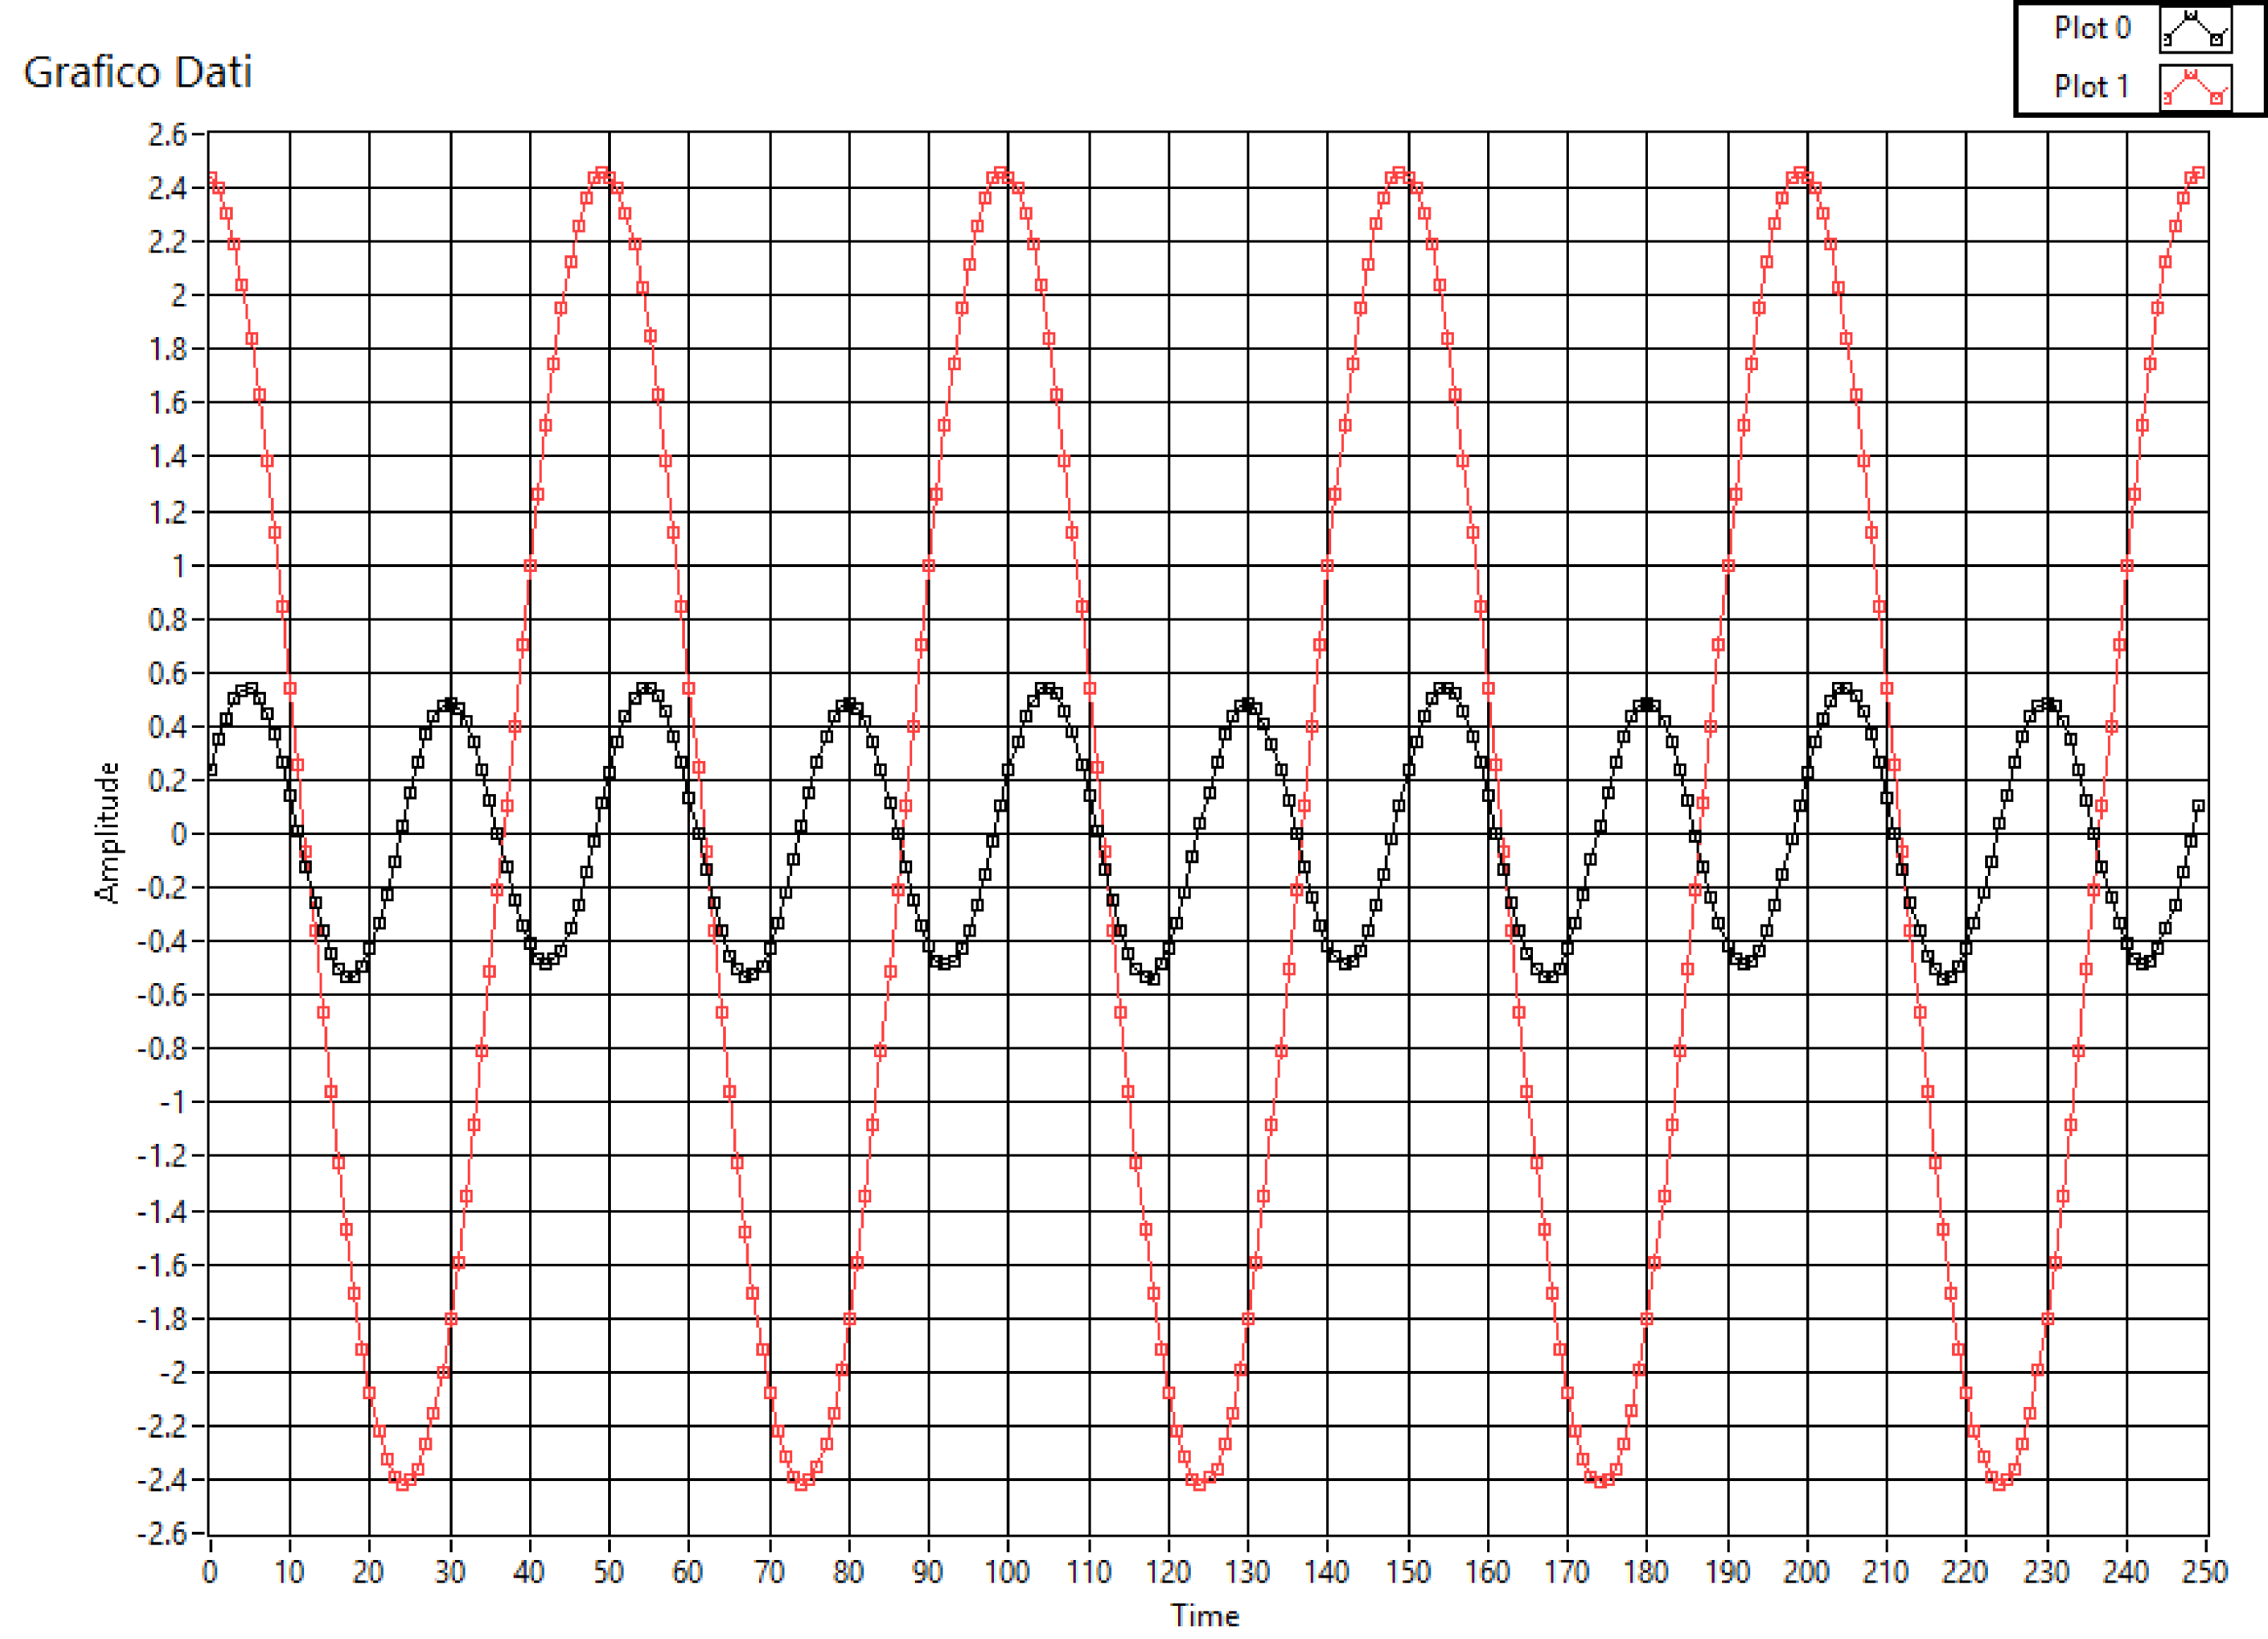
\includegraphics[width=0.5\linewidth]{./es20_part_1_11}
\label{fig:es20_fig2}}
%\qquad

\caption{Segnale in uscita rinforzato con partitori di diversa dimensione.}
\label{fig:es20_sub}
\end{figure}

\subsection{Misure del prodotto}


Si faccia riferimento alla figura \ref{fig:schema_ad633} per la configurazione dei pin nel AD633. Si vuole adesso configurare il circuito in modo tale da impiegare anche il canale B del generatore ATTEN. La configurazione immediata è naturalmente quella di mettere i pin 2 e 4 a terra, il pin 1 ad esempio al canale B dell'ATTEN e al pin 3 il canale A sempre del generatore. Se i segnali generati sono segnali sinusoidali della stessa frequenza ma sfasati fra loro, è facile vedere come il segnale in uscita dal dispositivo avrà un offset che dipende dalla fase relativa dei due segnali. Infatti se

\begin{gather}
V_A = A \sin (\omega t + \varphi) \\
V_B = B \sin (\omega t)
\end{gather}

sono i segnali inviati al dispositivo, il segnale in uscita è dato dalla formula che appare in figura \ref{fig:schema_ad633}, in questo caso:

\begin{equation}
\begin{split}
V_{out} & = C \sin (\omega t + \varphi) \sin (\omega t) \\
		& = \frac{C}{2} ( \cos \varphi - \cos (2 \omega t + \varphi))
\end{split}
\end{equation}

dove C = AB. Quindi la presenza di una fase relativa implica la comparsa di un offset, che è massimo quando la fase è nulla. È opportuno quindi avere un modo per avere sotto controllo la fase relativa dei segnali in ingresso al AD633. Fortunatamente il generatore ATTEN consente di regolare direttamente la fase dei segnali trasmessi tramite i due canali per mezzo di una opportuna combinazione di pulsanti. Un'alternativa è collegare ad uno dei segnali in ingresso un filtro (derivatore o integratore) che oltre ad un'attenuazione introduce una fase senza cambiare, nel caso di segnali puramente monocromatici, la forma dell'onda. In questo caso la fase si può regolare mettendo come resistenza un potenziometro.\\
È interessante considerare anche il caso in cui i due segnali non hanno esattamente la stessa frequenza, dal momento che questo è proprio il caso che si presenta impostando frequenze uguali per i due canali dell'ATTEN in quanto non ci si può naturalmente aspettare che questo sia effettivamente rispettato. Sempre per mezzo della formula di cui in figura \ref{fig:schema_ad633}, se i due segnali sono:

\begin{gather}
V_A = A \sin (\omega _1 t + \varphi) \\
V_B = B \sin (\omega _2 t)
\end{gather}

si ottiene:

\begin{equation}
\begin{split}
V_{out} & = C \sin (\omega _1 t + \varphi) \sin (\omega  _2 t ) \\
		& = \frac{C}{2} ( \cos ((\omega _1 - \omega _2 ) t + \varphi) - \cos ((\omega _1 + \omega _2) t + \varphi))
\end{split}
\end{equation}

Ovvero la somma di un segnale di frequenza $\omega _1 + \omega _2 \approx 2 \omega$ con un segnale di frequenza molto più piccola. Ciò che ci si aspetta di vedere è quindi un segnale di frequenza $2 \omega$ con un offset che varia periodicamente e lentamente. Questo è effettivamente quanto si è osservato (è disponibile su gentile concessione degli autori un video che lo dimostra).\\ Nelle figure  \ref{subfig2} i grafici restituiti dal VI \texttt{Acquis$\_$base4} al variare della fase dei due segnali in ingresso.

\begin{figure}[h]
\centering
\subfloat[$\Delta \varphi \approx 0^{\circ}$]{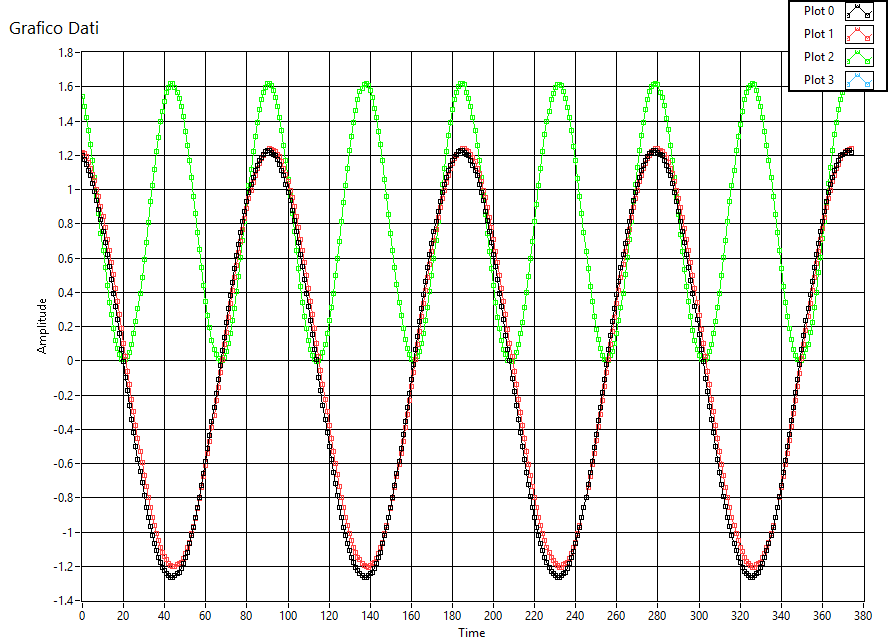
\includegraphics[width=0.5\linewidth]{es24_circa0grad}
\label{fig:tiger1}}
\subfloat[$\Delta \varphi \approx 80^{\circ}$]{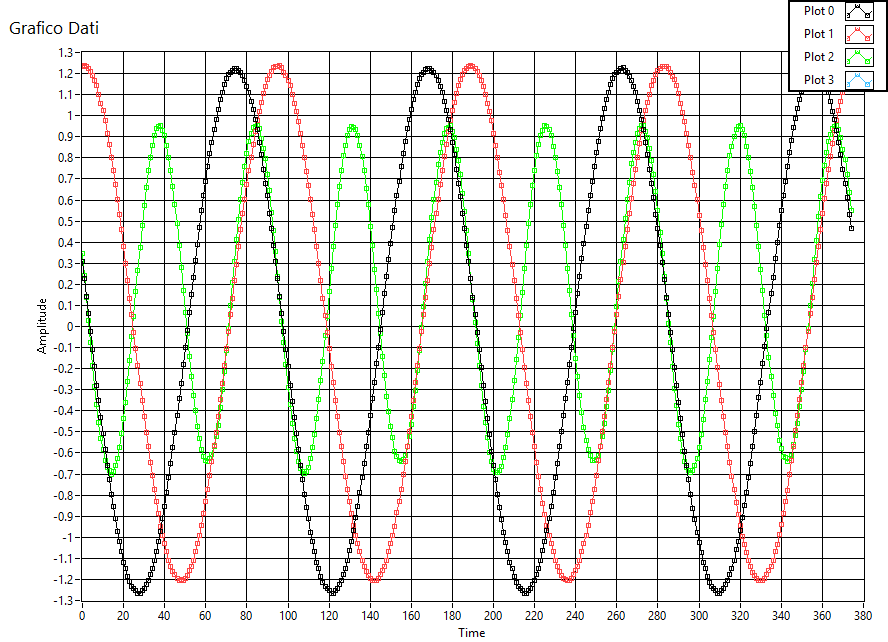
\includegraphics[width=0.5\linewidth]{es24_circa80grad}
%\caption{$\Delta \varphi \approx 80^{\circ}$}
\label{fig:mouse1}}
\qquad
\subfloat[$\Delta \varphi \approx 180^{\circ}$]{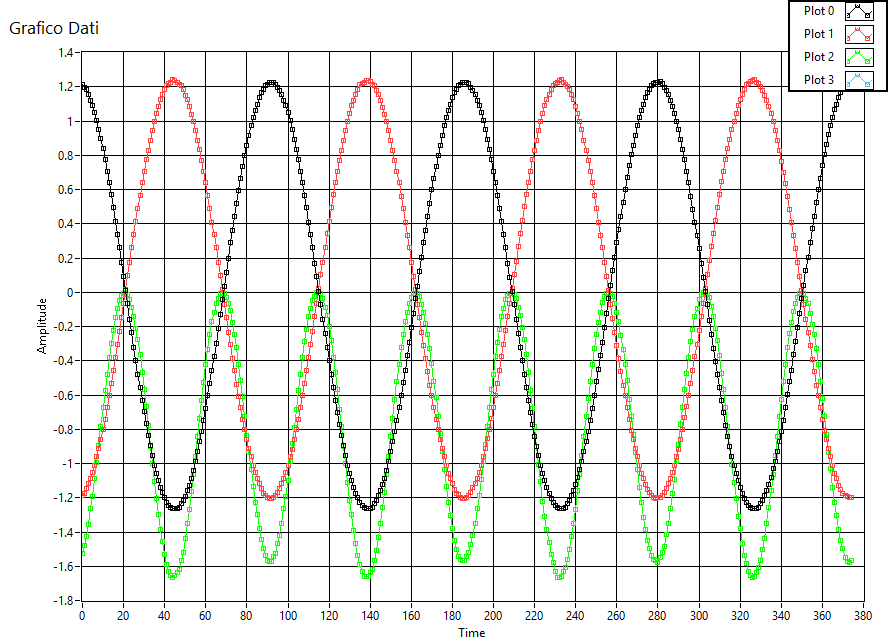
\includegraphics[width=0.5\linewidth]{es24_circa180grad}
%\caption{$\Delta \varphi \approx 180^{\circ}$}
\label{fig:mouse3}}
\subfloat[$\Delta \varphi \approx 220^{\circ}$]{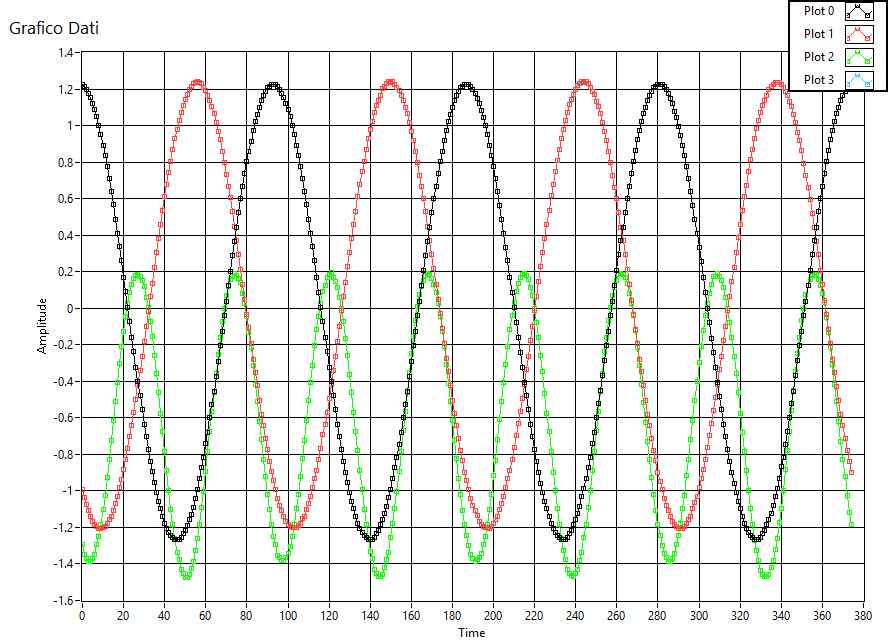
\includegraphics[width=0.5\linewidth]{es24_circa220grad}
\label{fig:gull}}
\caption{Uscita AD633 in funzione della fase relativa. In rosso e nero gli ingressi, in verde l'uscita}
\label{subfig2}
\end{figure}


Per misurare l'offset dovuto alla differenza di fase dei segnali in ingresso al AD633 è possibile servirsi del circuito in figura \ref{es26}.

\begin{figure}[!h]
\centering
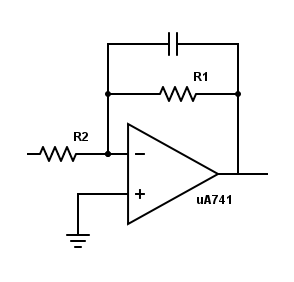
\includegraphics[scale=.6]{es25}
\caption{Schema del circuito "mediatore"}
\label{es26}
\end{figure}

Si ha che esso esegue una media del segnale in ingresso fatta su un tempo $\tau  = R_2C$, dopodichè il segnale mediato risulta moltiplicato per un fattore $-\frac{R_1}{R_2}$. Abbiamo scelto come valori delle impedenze C = 100nF, $R_1$ = 224 k$\Omega$, $R_2$ = 55.6 $\Omega$. Pertanto $\tau$=5.56 ms, circa 4 volte il periodo del segnale, $\tau_s$ = 1.25 ms, e un fattore di amplificazione di -4. In figura \ref{subfig3} sono mostrati i grafici restituiti da \texttt{Acquis$\_$base4}, si vede come effettivamente i risultati sono in accordo con quanto previsto.

\begin{figure}[h]
\centering
\subfloat[$\Delta \varphi \approx 0^{\circ}$]{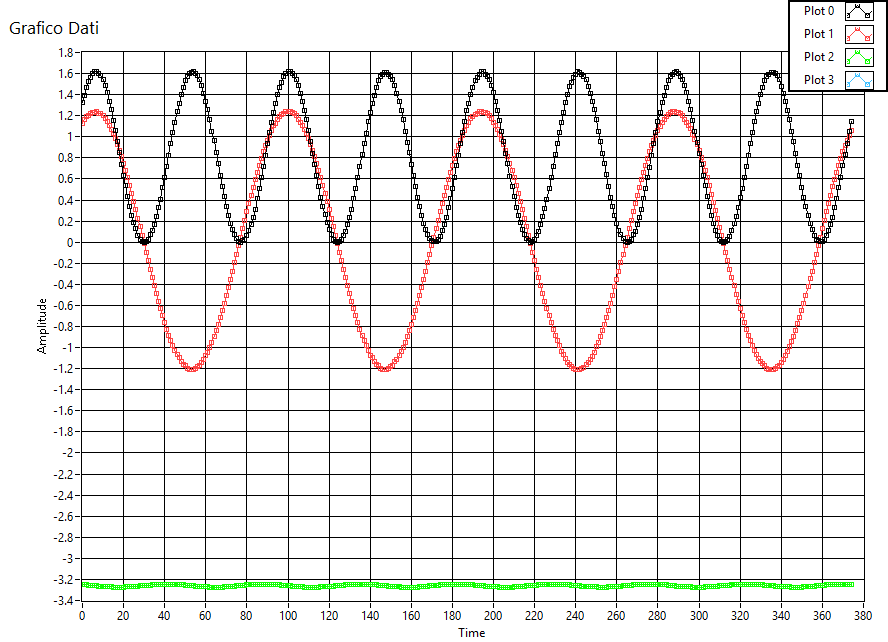
\includegraphics[width=0.5\linewidth]{es25_800hz_100nF_0deg}
\label{fig:tiger}}
\subfloat[$\Delta \varphi \approx 90^{\circ}$]{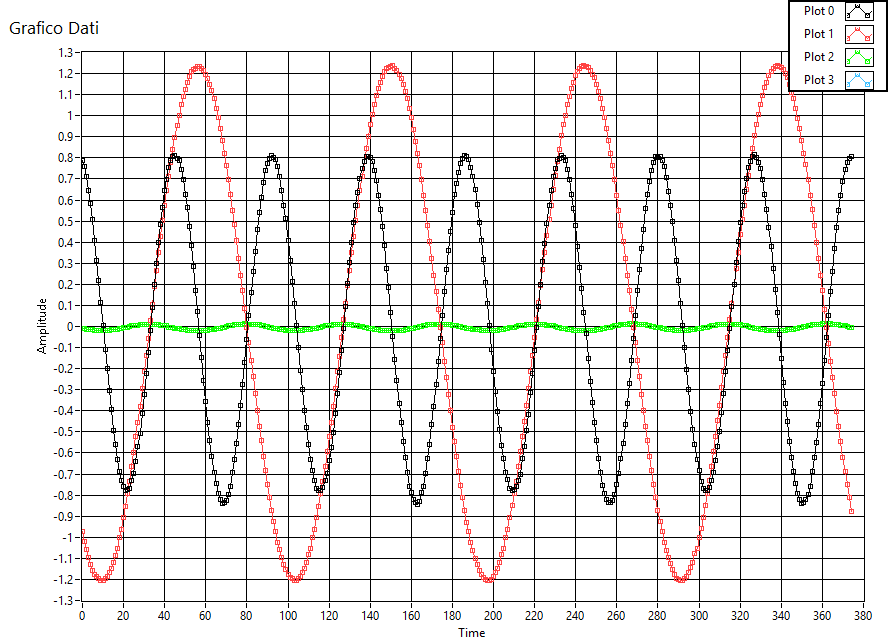
\includegraphics[width=0.5\linewidth]{es25_800hz_100nF_90deg}
\label{fig:mouse5}}
\qquad 
\subfloat[$\Delta \varphi \approx 180^{\circ}$]{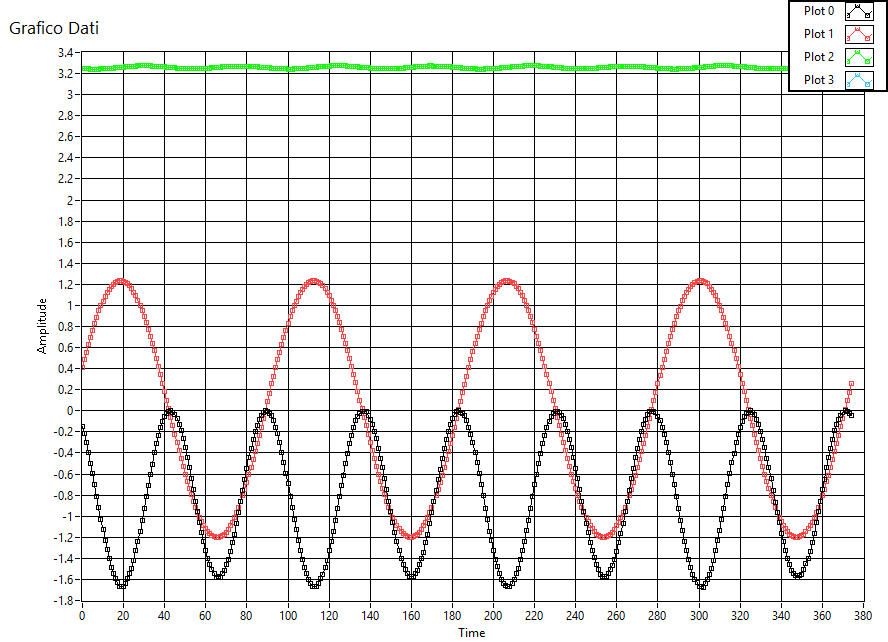
\includegraphics[width=0.5\linewidth]{es25_800hz_100nF_180deg}
\label{fig:mouse25}}
   
\caption{Uscita AD633 in funzione della fase relativa. In rosso uno dei due segnali in ingresso, in nero l'uscita dal AD633, in verde l'uscita dal mediatore}
\label{subfig3}
\end{figure}


\begin{thebibliography}{10}
\bibitem{bib1}
Lorem M, Ipsum VE (1990) Rank Correlation Methods. New York: Oxford University Press, 5th edition.

\bibitem{bib2}
Ipsum M, Ipsum JD (1990) Rank Correlation Methods. New York: Oxford University Press, 5th edition.

\end{thebibliography}



\end{document}